% This is "sig-alternate.tex" V2.1 April 2013
% This file should be compiled with V2.5 of "sig-alternate.cls" May 2012
%
% This example file demonstrates the use of the 'sig-alternate.cls'
% V2.5 LaTeX2e document class file. It is for those submitting
% articles to ACM Conference Proceedings WHO DO NOT WISH TO
% STRICTLY ADHERE TO THE SIGS (PUBS-BOARD-ENDORSED) STYLE.
% The 'sig-alternate.cls' file will produce a similar-looking,
% albeit, 'tighter' paper resulting in, invariably, fewer pages.
%
% ----------------------------------------------------------------------------------------------------------------
% This .tex file (and associated .cls V2.5) produces:
%       1) The Permission Statement
%       2) The Conference (location) Info information
%       3) The Copyright Line with ACM data
%       4) NO page numbers
%
% as against the acm_proc_article-sp.cls file which
% DOES NOT produce 1) thru' 3) above.
%
% Using 'sig-alternate.cls' you have control, however, from within
% the source .tex file, over both the CopyrightYear
% (defaulted to 200X) and the ACM Copyright Data
% (defaulted to X-XXXXX-XX-X/XX/XX).
% e.g.
% \CopyrightYear{2007} will cause 2007 to appear in the copyright line.
% \crdata{0-12345-67-8/90/12} will cause 0-12345-67-8/90/12 to appear in the copyright line.
%
% ---------------------------------------------------------------------------------------------------------------
% This .tex source is an example which *does* use
% the .bib file (from which the .bbl file % is produced).
% REMEMBER HOWEVER: After having produced the .bbl file,
% and prior to final submission, you *NEED* to 'insert'
% your .bbl file into your source .tex file so as to provide
% ONE 'self-contained' source file.
%
% ================= IF YOU HAVE QUESTIONS =======================
% Questions regarding the SIGS styles, SIGS policies and
% procedures, Conferences etc. should be sent to
% Adrienne Griscti (griscti@acm.org)
%
% Technical questions _only_ to
% Gerald Murray (murray@hq.acm.org)
% ===============================================================
%
% For tracking purposes - this is V2.0 - May 2012

\documentclass{sig-alternate-05-2015}

\usepackage{pifont} 
\usepackage{import}
\usepackage{amsmath}
\usepackage{multirow}
\usepackage{graphicx,url}
\usepackage{placeins}
\usepackage{adjustbox}
\usepackage[english]{babel}
\usepackage{lipsum}
\usepackage{multicol}
\usepackage{listings}
\usepackage[svgnames]{xcolor} 
\usepackage{caption}
\usepackage{amsmath}
\usepackage{calc} 
\usepackage{array,url,kantlipsum}
\usepackage{lscape}
\usepackage{array}
\usepackage{booktabs}
\usepackage{txfonts}
\usepackage{colortbl}%
  \newcommand{\myrowcolour}{\rowcolor[gray]{0.925}}
\newenvironment{Figure}
  {\par\medskip\noindent\minipage{\linewidth}}
  {\endminipage\par\medskip}
  
\DeclareCaptionFont{white}{\color{white}}
\DeclareCaptionFormat{listing}{\colorbox[RGB]{60,100,180}{\parbox{0.40\textwidth - 2 \fboxsep}{\hspace{8pt}#1#2#3}}}
\captionsetup[lstlisting]{format=listing,labelfont=white,textfont=white, singlelinecheck=false, margin=0pt, font={bf,footnotesize}}


\begin{document}





% Copyright
\setcopyright{acmcopyright}
%\setcopyright{acmlicensed}
%\setcopyright{rightsretained}
%\setcopyright{usgov}
%\setcopyright{usgovmixed}
%\setcopyright{cagov}
%\setcopyright{cagovmixed}


% DOI
\doi{10.475/123_4}

% ISBN
\isbn{123-4567-24-567/08/06}

%Conference
\conferenceinfo{PLDI '13}{June 16--19, 2013, Seattle, WA, USA}

\acmPrice{\$15.00}

%
% --- Author Metadata here ---
\conferenceinfo{SBST}{'06 Austin, Texas USA}
%\CopyrightYear{2007} % Allows default copyright year (20XX) to be over-ridden - IF NEED BE.
%\crdata{0-12345-67-8/90/01}  % Allows default copyright data (0-89791-88-6/97/05) to be over-ridden - IF NEED BE.
% --- End of Author Metadata ---

\title{Improving Load, Performance and Stress Search Based Testing using a Hybrid Metaheuristic Approach}
%\subtitle{[Extended Abstract]
%\titlenote{A full version of this paper is available as
%\textit{Author's Guide to Preparing ACM SIG Proceedings Using
%\LaTeX$2_\epsilon$\ and BibTeX} at
%\texttt{www.acm.org/eaddress.htm}}}
%
% You need the command \numberofauthors to handle the 'placement
% and alignment' of the authors beneath the title.
%
% For aesthetic reasons, we recommend 'three authors at a time'
% i.e. three 'name/affiliation blocks' be placed beneath the title.
%
% NOTE: You are NOT restricted in how many 'rows' of
% "name/affiliations" may appear. We just ask that you restrict
% the number of 'columns' to three.
%
% Because of the available 'opening page real-estate'
% we ask you to refrain from putting more than six authors
% (two rows with three columns) beneath the article title.
% More than six makes the first-page appear very cluttered indeed.
%
% Use the \alignauthor commands to handle the names
% and affiliations for an 'aesthetic maximum' of six authors.
% Add names, affiliations, addresses for
% the seventh etc. author(s) as the argument for the
% \additionalauthors command.
% These 'additional authors' will be output/set for you
% without further effort on your part as the last section in
% the body of your article BEFORE References or any Appendices.

\numberofauthors{4} %  in this sample file, there are a *total*
% of EIGHT authors. SIX appear on the 'first-page' (for formatting
% reasons) and the remaining two appear in the \additionalauthors section.
%
\author{
% You can go ahead and credit any number of authors here,
% e.g. one 'row of three' or two rows (consisting of one row of three
% and a second row of one, two or three).
%
% The command \alignauthor (no curly braces needed) should
% precede each author name, affiliation/snail-mail address and
% e-mail address. Additionally, tag each line of
% affiliation/address with \affaddr, and tag the
% e-mail address with \email.
%
% 1st. author
\alignauthor
Francisco Nauber Bernardo Gois\\
     \affaddr{Servi\c{c}o Federal de Processamento de Dados}\\
       \affaddr{Avenida Pontes Vieria ,832}\\
       \affaddr{Fortaleza, Cear\'a, Brazil}\\
       \email{francisco.gois@serpro.gov.br}
% 2nd. author
\alignauthor
Pedro Porf\'irio Muniz de Farias\\
       \affaddr{Universidade de Fortaleza}\\
       \affaddr{Av. Washington Soares, 1321}\\
       \affaddr{Fortaleza, Cear\'a, Brazil}\\
       \email{porfirio@unifor.br}
% 3rd. author
\alignauthor Andr\'e Lu\'is Vasconcelos Coelho\\
       \affaddr{Universidade de Fortaleza}\\
       \affaddr{Av. Washington Soares, 1321}\\
       \affaddr{Fortaleza, Cear\'a, Brazil}\\
       \email{acoelho@unifor.br}
\and  % use '\and' if you need 'another row' of author names
% 4th. author
\alignauthor Thiago Monteiro Barbosa\\
       \affaddr{Servi\c{c}o Federal de Processamento de Dados}\\
       \affaddr{Avenida Pontes Vieria ,832}\\
       \affaddr{Fortaleza, Cear\'a, Brazil}\\
       \email{thiago.barbosa@serpro.gov.br}
}

\additionalauthors{Additional authors: Thiago Monteiro Barbosa (Servi\c{c}o Federal de Processamento de Dados,
email: {\texttt{thiago.barbosa@serpro.gov.br}}) .}


\maketitle
\begin{abstract}
 Some software systems must respond to thousands or millions of concurrent requests. These systems must be properly tested to ensure that they can function correctly under the expected load. Load, performance, and stress search-based testing aim to find test scenarios that produce execution times that violate the timing constraints specified. The purpose of this paper is to identify test scenarios that exercise a system in a way that tasks are pushed as close as possible to their limits. The research proposes a hybrid metaheuristic approach that uses genetic algorithms, simulated annealing, and Tabu search algorithms for use in load, performance, and stress test models. A tool named IAdapter, a JMeter plugin used for performing search-based load, performance, or stress tests, was developed. Two experiments were conducted to validate the proposed approach. The first experiment was performed on an emulated component, and the second one was performed using an installed Moodle application. In both experiments, the use of a hybrid metaheuristic approach produced better fitness values. 
\end{abstract}


%
% The code below should be generated by the tool at
% http://dl.acm.org/ccs.cfm
% Please copy and paste the code instead of the example below. 
%
\begin{CCSXML}
<ccs2012>
<concept>
<concept_id>10011007.10011074.10011099</concept_id>
<concept_desc>Software and its engineering~Software verification and validation</concept_desc>
<concept_significance>500</concept_significance>
</concept>
</ccs2012>
\end{CCSXML}

\ccsdesc[500]{Software and its engineering~Software verification and validation}


\widowpenalties 1 10000
\raggedbottom

%
% End generated code
%

%
%  Use this command to print the description
%
\printccsdesc

% We no longer use \terms command
%\terms{Theory}

\keywords{Search-Based Testing;Tabu Search;Hybrid Metaheuristics}

\section{Introduction}

Many systems must support concurrent access by hundreds or thousands of users. Failure to scale users results in catastrophic failures and unfavorable media coverage \cite{Jiang2010}. To ensure the quality of these systems, it is necessary to perform a testing procedure such as performance, stress, and load testing \cite{Jiang2009}. 

The explosive growth of the Internet has contributed to the increased need for applications that perform at an appropriate speed. Performance problems are often detected late in the application life cycle, and the later they are discovered, the greater the cost to fix them \cite{Molyneaux2009}.
% * <naubergois@gmail.com> 2015-09-16T23:58:29.774Z:
%
%  Alterar frase
%
% ^ <naubergois@gmail.com> 2015-09-16T23:58:46.491Z.
% * <naubergois@gmail.com> 2015-09-16T23:58:52.202Z:
%
% 
%
The use of load testing is an increasingly common practice owing to the increasing number of users. In this scenario, the inadequate treatment of a workload generated by concurrent or simultaneous access, generated by system users, can result in highly critical failures and negatively affect the customers's perception of the company \cite{Draheim2006b} \cite{Jiang2010}. 

Load testing determines the responsiveness, throughput, reliability, or scalability of a system under a given workload. The quality of the results of a system's load tests is closely linked to the implementation of the workload strategy. The performance of many applications depends on the load applied under different conditions. In some cases, performance degradation and failures arise only in stress conditions \cite{Garousi2010} \cite{Jiang2010}.

A load, performance, or stress test uses a set of workloads that consist of many types of usage scenarios and a combination of different numbers of users. A load is typically based on an operational profile. Different parts of an application should be tested on various parameters and stress conditions \cite{Babbar2011}. The correct application of a load test should cover most parts of an application under ordinary conditions (load or performance test) or above the expected load conditions (stress test)\cite{Draheim2006b} \cite{Luiz2011} \cite{Fe2004}.

Fig. \ref{fig:example} shows an example of a system under test with three pages (the main page, profile page, and search page) and six possible users. From the combinations of users and application pages, various scenarios can be created such as scenarios 1 and 2 shown in the figure. The first scenario presents a test that has passed, and the second scenario presents a test that has an HTTP error of 404.

\begin{figure}[ht]
\centering
\caption{Possible test scenarios for a hypothetical application}
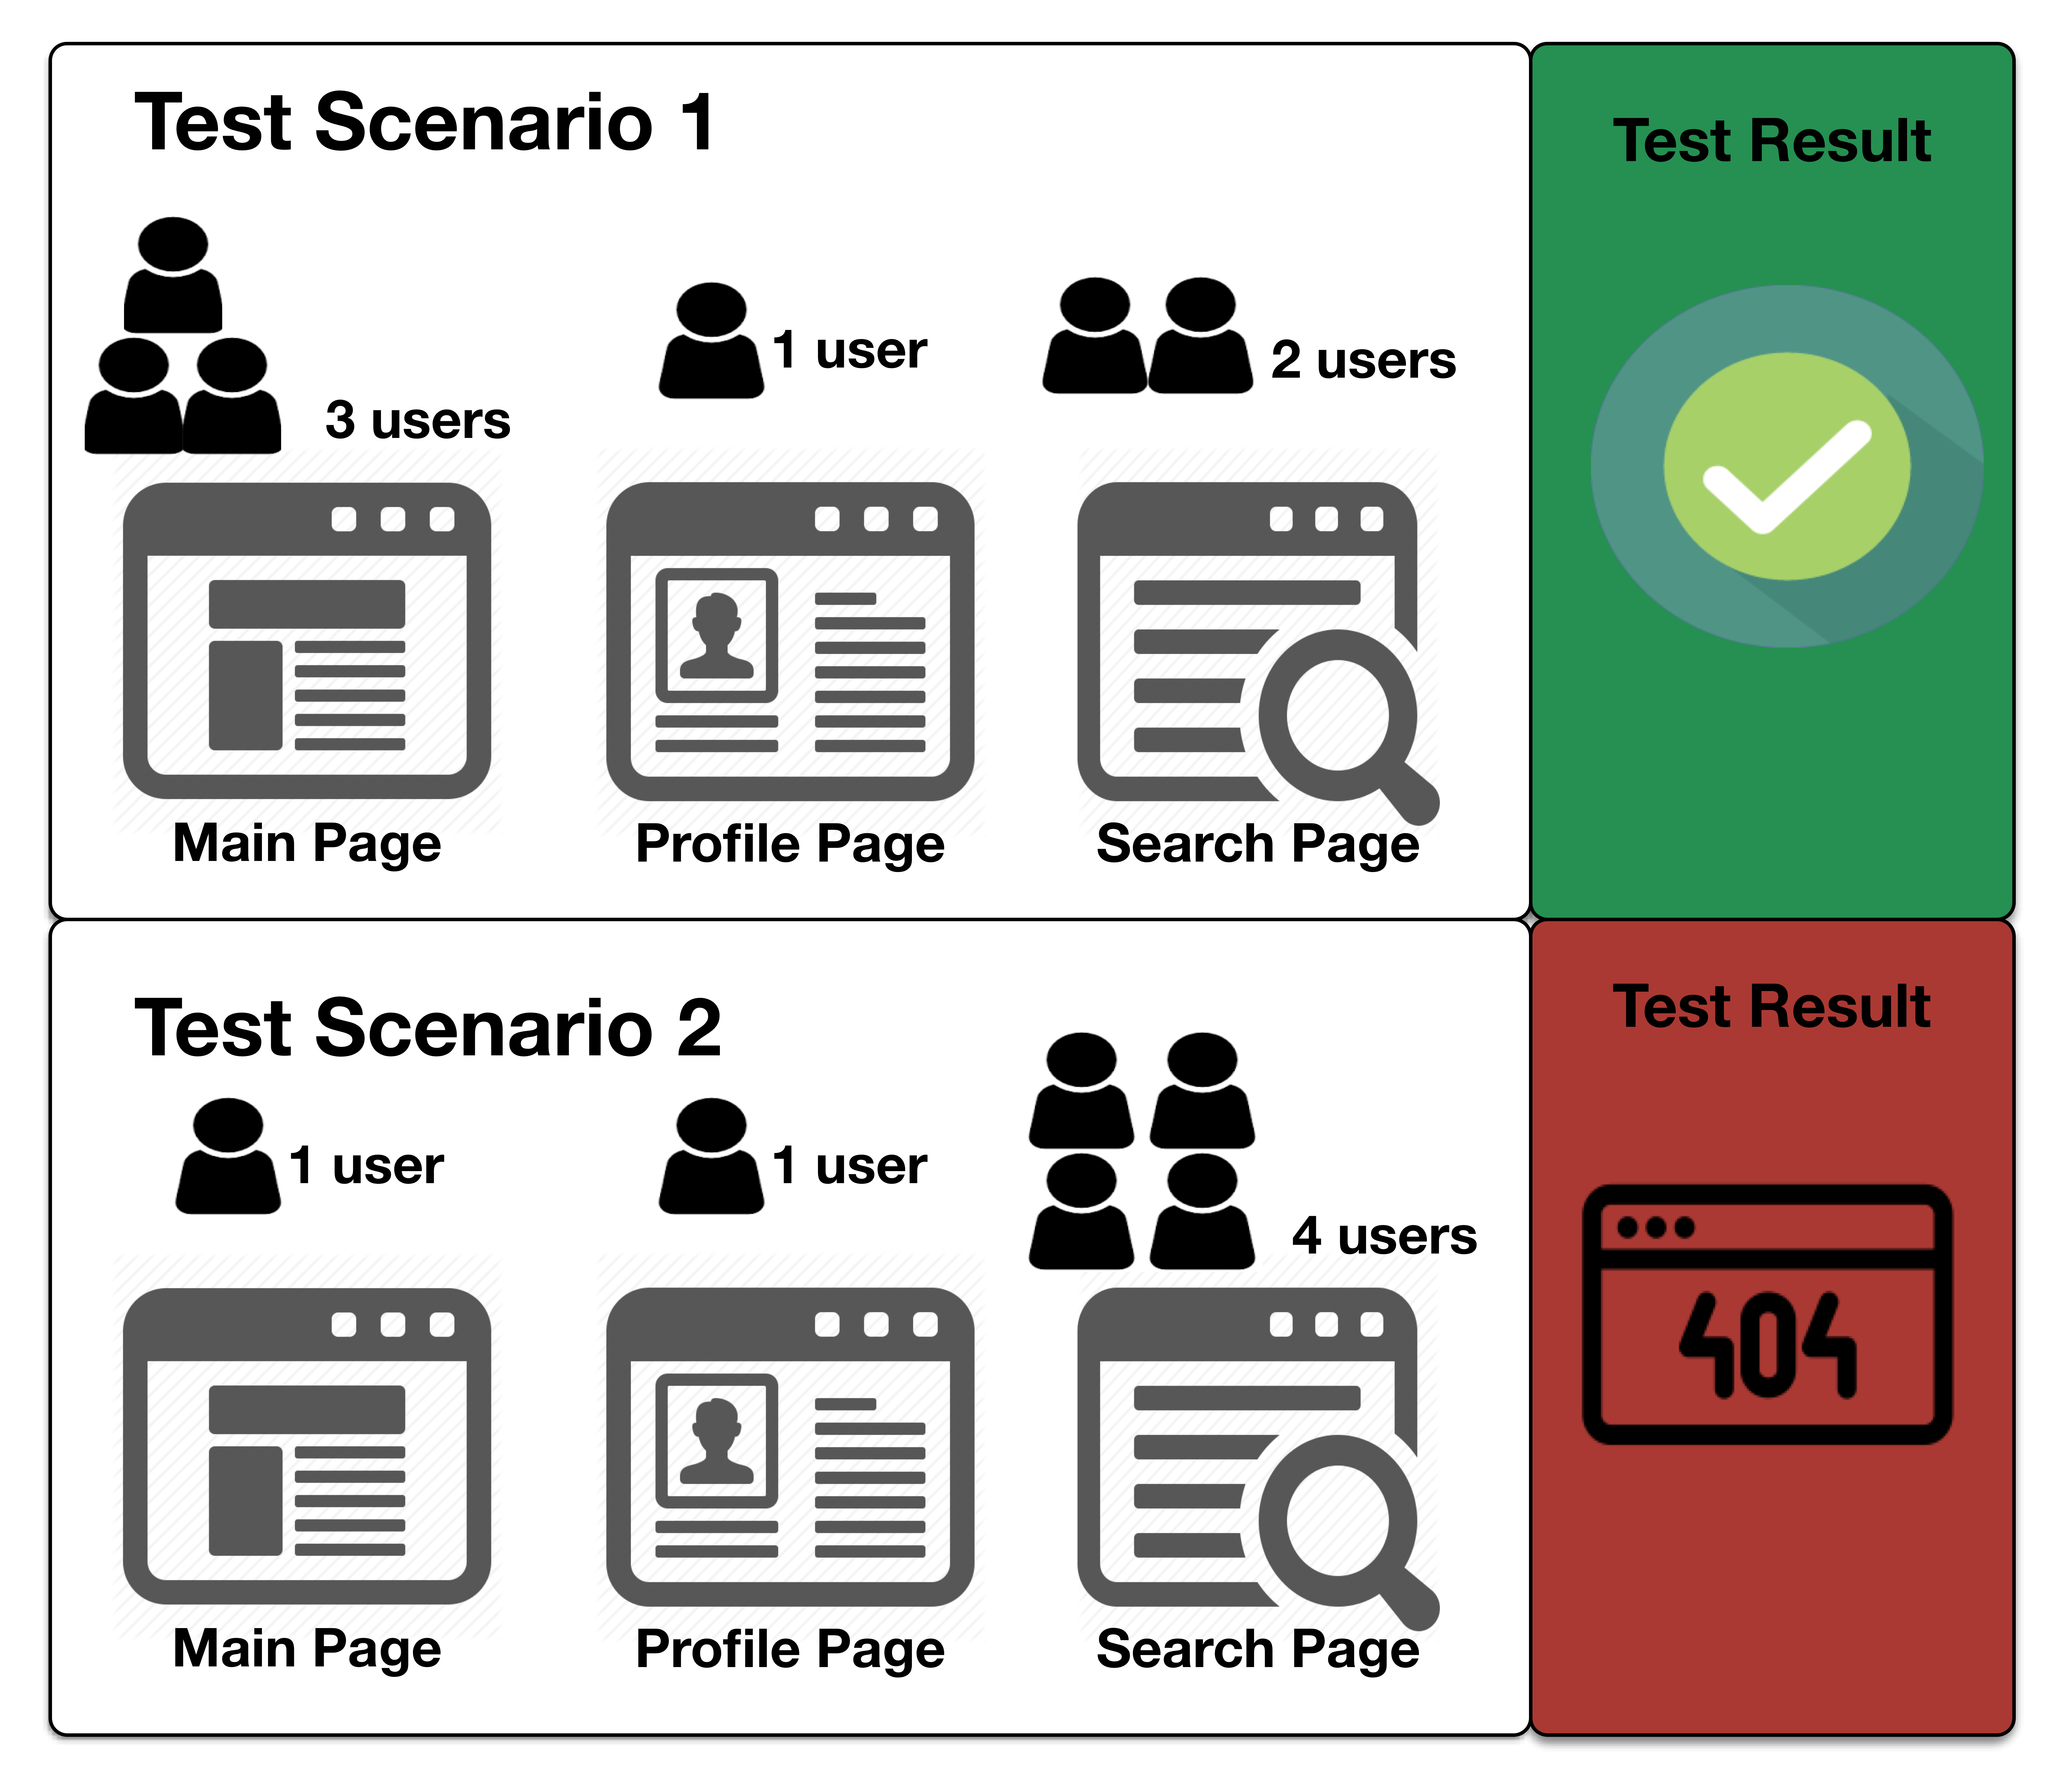
\includegraphics[width=0.4\textwidth]{./images/diagram.png}
\label{fig:example}
\end{figure}

A performance test usually lasts for several hours or even a few days and only tests a limited number of workloads. The major challenge is to find the workloads that expose a major number of errors and to discover the maximum number of users supported by an application under test \cite{Barna2011}. 

Search-based test is seen as a promising approach for verifying timing constraints \cite{Afzal2009a}. The main objective of a load, performance, and stress search-based test is to find test scenarios that produce execution times that violate the specified timing constraints \cite{Sullivan}. 

The main objective of this research is to find test scenarios that maximize the likelihood of task deadline misses. Fig. \ref{fig:solution} presents an illustrative example where the presented research work approach finds test scenarios that expose errors or response times exceeding the maximum response time expected. There are many benefits in the use of the solution:


\begin{itemize}
\item It generates stress test cases that maximize the likelihood of task deadline misses.
\item  It automates the search for failure points of an application under test.
\end{itemize}



\begin{figure}[ht]
\centering
\caption{Illustrative example of the use of the presented research work approach}
\includegraphics[width=0.25\textwidth]{./images/solution.png}
\label{fig:solution}
\end{figure}

The paper proposes the use of a hybrid metaheuristic approach that combines genetic algorithms, simulated annealing, and Tabu search algorithms in load, performance, and stress evolutionary tests.

A tool named IAdapter, a JMeter plugin for performing search-based load, performance, or stress tests, was developed. Two experiments were conducted to validate the proposed approach. The first experiment was performed on an emulated component, and the second one was performed using an installed Moodle application.

The remainder of the paper is organized as follows. Section 2 presents a brief introduction about load, performance, and stress tests. Section 3 presents concepts about the workload model. Section 4 presents concepts about hybrid metaheuristic algorithms. Section 5 presents the research-proposed approach. Section 6 presents the IAdapter tool. Section 7 discusses the related work. Section 8 shows the results of two experiments performed using the IAdapter plugin. Conclusions and further work are presented in Section 9.




\section{Load, Performance and Stress Test}

Load, performance, and stress testing are typically done to locate bottlenecks in a system, to support a performance-tuning effort, and to collect other performance-related indicators to help stakeholders get informed about the quality of the application being tested \cite{Sandler2004} \cite{Corporation2007}. 

The performance test aims at verifying a specified system performance. This kind of test is executed by simulating hundreds of simultaneous users or more over a defined time interval \cite{DiLucca2006}. The purpose of this test is to demonstrate that the system reaches its performance objectives \cite{Sandler2004}. 


In a load test, the system is evaluated at predefined load levels \cite{DiLucca2006}. The aim of this test is to determine whether the system can reach its performance targets for availability, concurrency, throughput, and response time. Load test is the closest to real application use \cite{Molyneaux2009}.

The stress test verifies the system behavior against heavy workloads \cite{Sandler2004}, which are executed to evaluate a system beyond its limits, validate system response in activity peaks, and verify whether the system is able to recover from these conditions. It differs from other kinds of testing in that the system is executed on or beyond its breakpoints, forcing the application or the supporting infrastructure to fail \cite{DiLucca2006} \cite{Molyneaux2009}.

Automated tools are needed to carry out serious load, stress, and performance testing. Sometimes, there is simply no practical way to provide reliable, repeatable performance tests without using some form of automation. The aim of any automated test tool is to simplify the testing process \cite{Molyneaux2009}.

In the context of testing, a scenario is a sequence of steps in an application. It can represent a use case or a business function such as searching a product catalog, adding an item to a shopping cart, or placing an order \cite{Corporation2007}. 

Load, performance, and stress results are measured by indicators. Some researchers advocate that the 90-percentile response time is a better measurement than the average/medium response time, as the former accounts for most of the peaks, while eliminating the outliers \cite{Jiang2010}.


\section{WorkLoad Model}

Load, performance, or stress testing projects should start with the development of a model for user workload that an application receives. This should take into consideration various performance aspects of the application and the infrastructure that a given workload will impact. A workload is a key component of such a model \cite{Molyneaux2009}.

The term \'{}workload\'{} represents the size of the demand that will be imposed on the application under test in an execution. The metric unit used for defining a workload is dependent on the application domain, such as the length of the video in a transcoding application for multimedia files or the size of the input files in a file compression application \cite{Feitelson2013} \cite{Molyneaux2009} \cite{Goncalves2014}. 

Workload is also defined by the distribution of load between the identified transactions at a given time. Workload helps researchers study the system behavior identified in several load models. A workload model can be designed to verify the predictability, repeatability, and scalability of a system \cite{Feitelson2013} \cite{Molyneaux2009}.


Workload modeling is the attempt to create a simple and general model that can then be used to generate synthetic workloads. The goal is typically to be able to create workloads that can be used in performance evaluation studies. Sometimes, the synthetic workload is supposed to be similar to those that occur in practice in real systems \cite{Feitelson2013} \cite{Molyneaux2009}.

There are two kinds of workload models: descriptive and generative. The difference between the two is that descriptive models just try to mimic the phenomena observed in the workload, whereas generative models try to emulate the process that generated the workload in the first place \cite{DiLucca2006}. 

In descriptive models, one finds different levels of abstraction on the one hand and different levels of fidelity to the original data on the other hand. The most strictly faithful models try to mimic the data directly using the statistical distribution of the data. The most common strategy used in descriptive modeling is to create a statistical model of an observed workload (Fig. \ref{fig:descriptivemodel}). This model is applied to all the workload attributes, e.g., computation, memory usage, I/O behavior, communication, etc. \cite{DiLucca2006}. Fig. \ref{fig:descriptivemodel} shows a simplified workflow of a descriptive model. The workflow has six phases. In the first phase, the user uses the system in the production environment. In the second phase, the tester collects the user's data, such as logs, clicks, and preferences, from the system. The third phase consists in developing a model designed to emulate the user's behavior. The fourth phase is made up of the execution of the test, emulation of the user's behavior, and log gathering.



\begin{figure}[!ht]
\centering
\includegraphics[width=0.4\textwidth]{./images/workloadmodel1.png}
\caption{Workload modeling based on statistical data \cite{DiLucca2006}}
\label{fig:descriptivemodel}
\end{figure}

Generative models are indirect in the sense that they do not model the statistical distributions. Instead, they describe how users will behave when they generate the workload. An important benefit of the generative approach is that it facilitates manipulations of the workload. It is often desirable to be able to change the workload conditions as part of the evaluation. Descriptive models do not offer any option regarding how to do so. With the generative models, however, we can modify the workload-generation process to fit the desired conditions \cite{DiLucca2006}. The difference between the workflows of the descriptive and the generative models is that user behavior is not collected from logs, but simulated from a model that can receive feedback from the test execution (Fig. \ref{fig:generativemodel}).

\begin{figure}[!ht]
\centering
\includegraphics[width=0.4\textwidth]{./images/workloadmodel2.png}
\caption{Workload modeling based on the generative model \cite{DiLucca2006}}
\label{fig:generativemodel}
\end{figure}



\section{Hybrid  Metaheuristic}


A large number of researchers have recognized the advantages and huge potential of building hybrid mathematical programming methods and metaheuristics. The main motivation for creating hybrid metaheuristics is to exploit the complementary character of different optimization strategies. In fact, choosing an adequate combination of algorithms can be the key to achieving top performance in solving many hard optimization problems \cite{Puchinger2005} \cite{Blum2012}.

There are two main categories of metaheuristic combinations: collaborative combinations and integrative combinations. These are presented in Fig. \ref{fig:metaheuristc} \cite{Raidl2006}.

\begin{figure}[h]
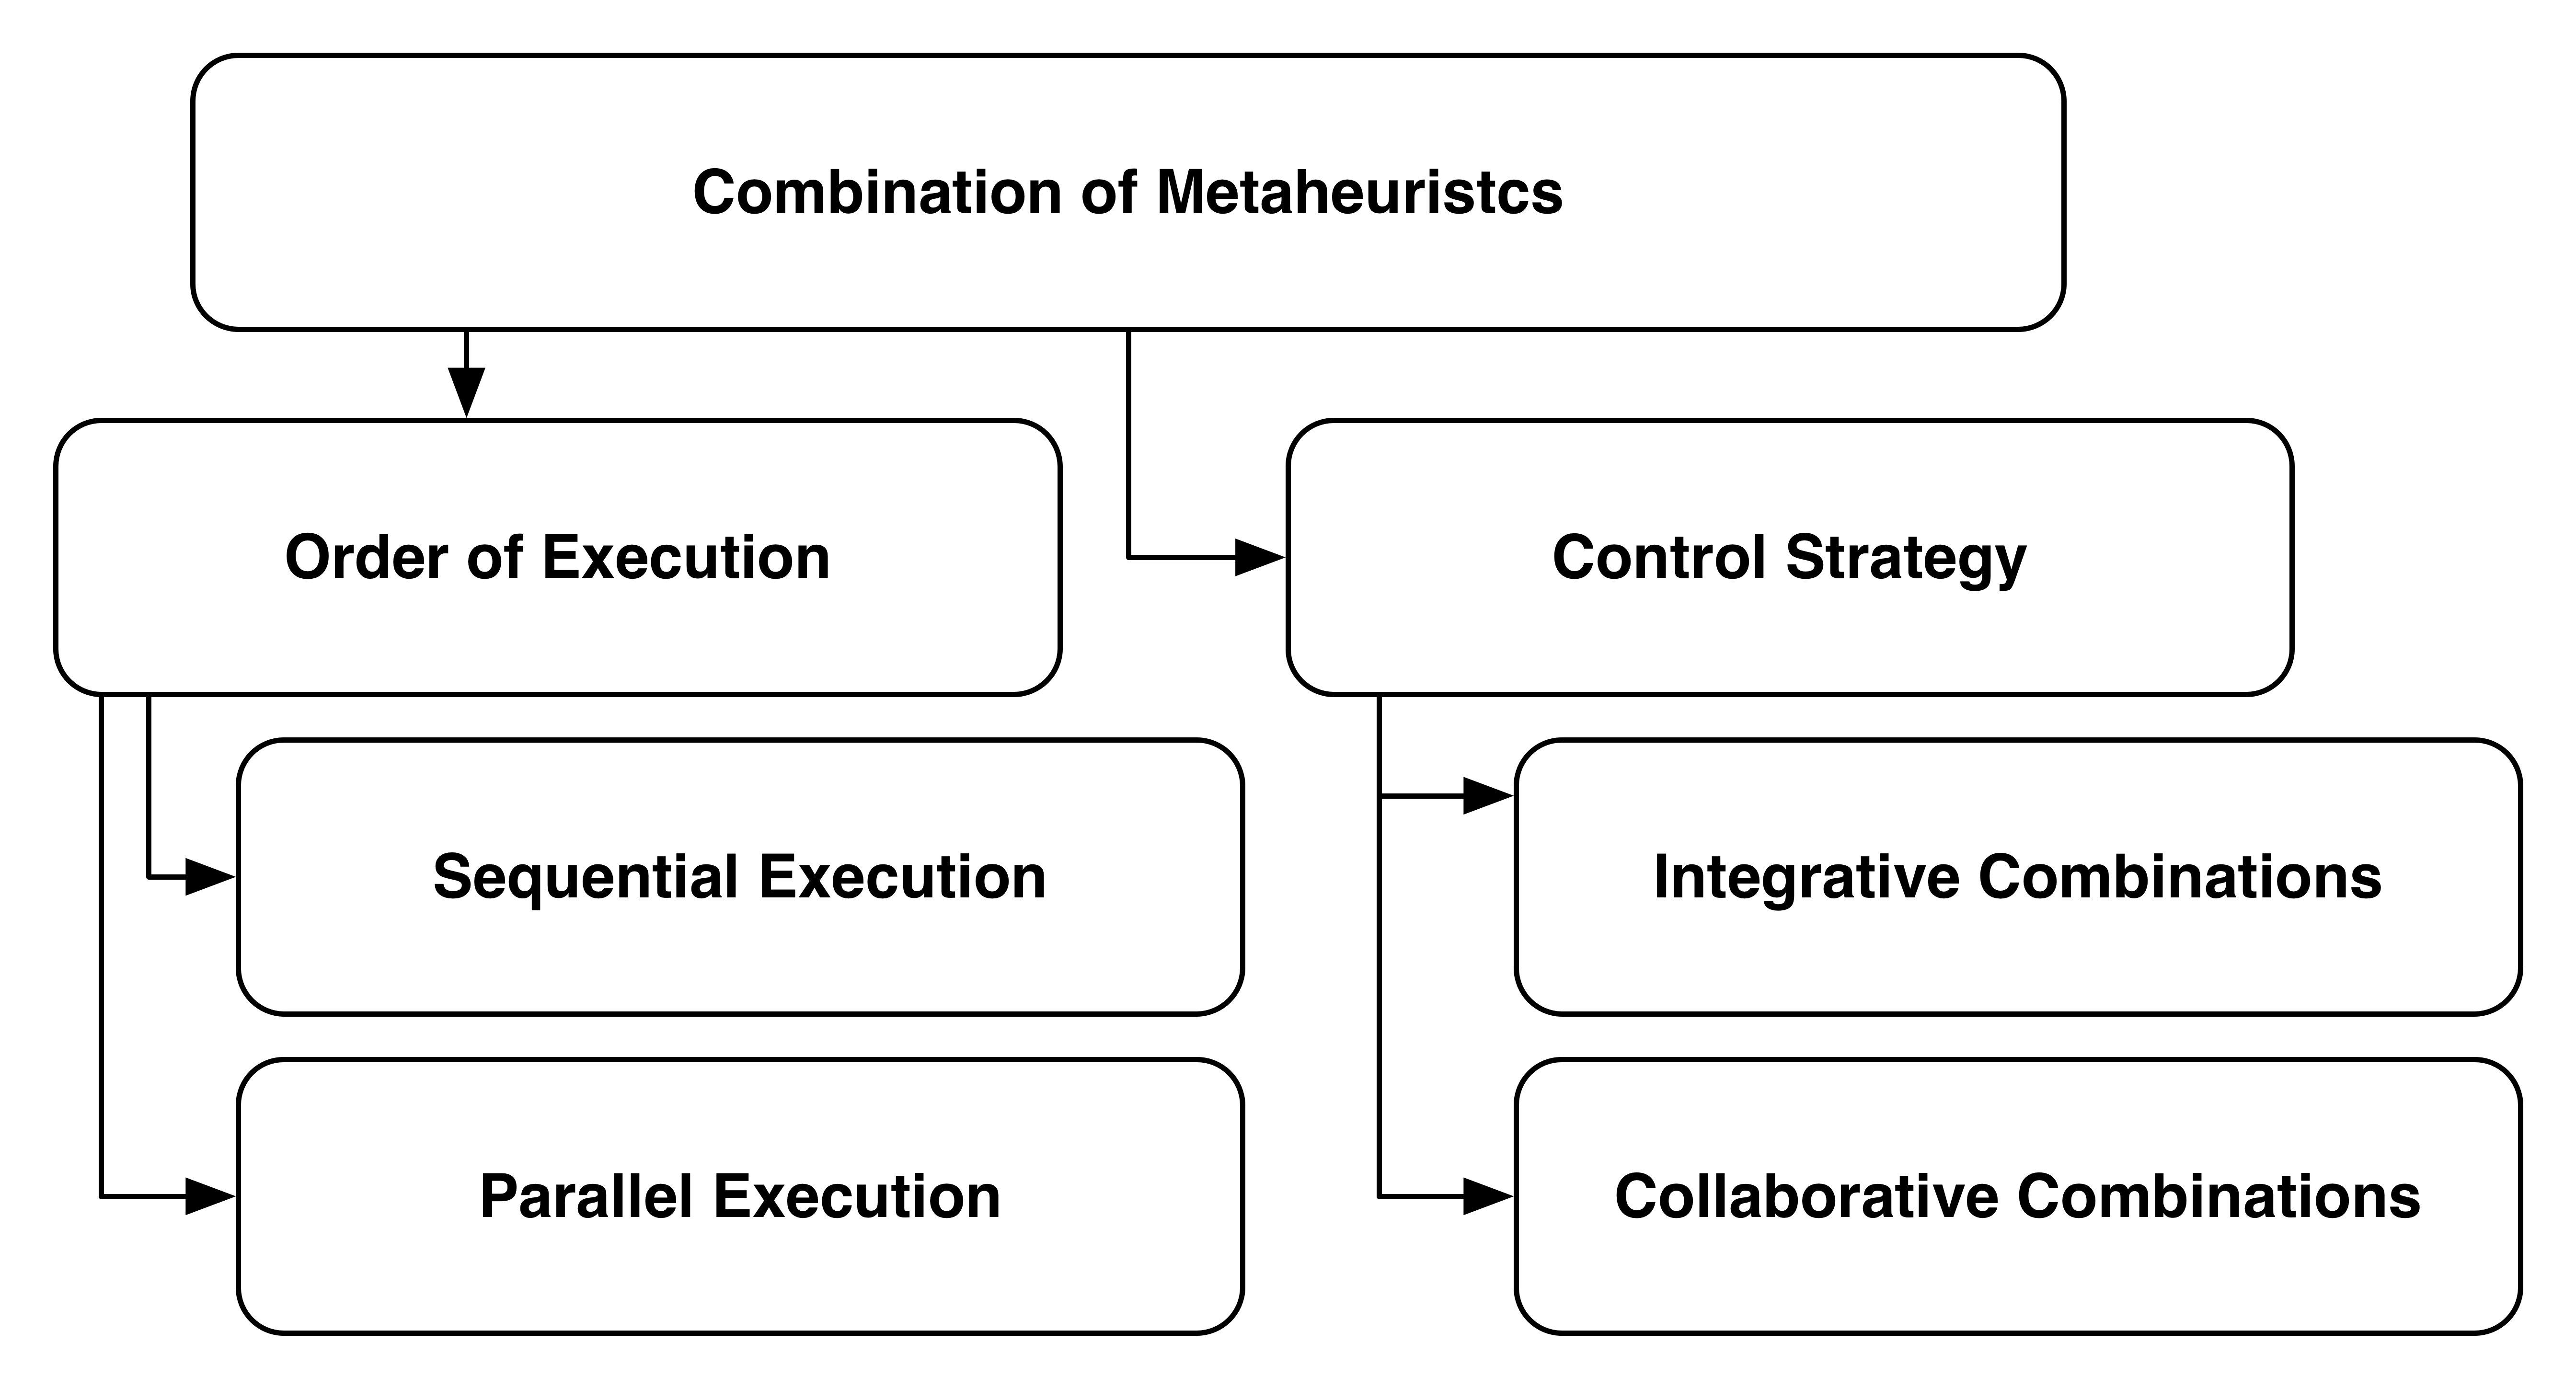
\includegraphics[width=0.5\textwidth]{./images/metaheuristc2.png}
\caption{Categories of metaheuristc combinations \cite{Puchinger2005} }
\label{fig:metaheuristc}
\end{figure}

Collaborative combinations use an approach where the algorithms exchange information, but are not part of each other. In this approach, algorithms may be executed sequentially or in parallel. The presented research work uses a type of collaborative combination with sequential execution.


\section{Improving Load, Performance, and Stress Search-Based Testing Using a Hybrid Metaheuristic Approach}


The proposed solution makes it possible to create a generative model that evolves during the test. The proposed solution model uses genetic algorithms, Tabu search, and simulated annealing in two different approaches. The first approach uses the three algorithms independently, and the second approach uses the three algorithms collaboratively (hybrid metaheuristic approach).

In the first approach , the algorithms do not share their best individuals among themselves. Each algorithm evolves in a separate way (Fig. \ref{fig:firstaproach}). The second approach uses the algorithms in a collaborative mode (hybrid metaheuristic). In this approach, the three algorithms share their best individuals found (Fig. \ref{fig:secondapproach}).

The next subsections present details about the used metaheuristic algorithms (genotype representation and fitness function) and the IAdapter components.

\begin{figure}[h]
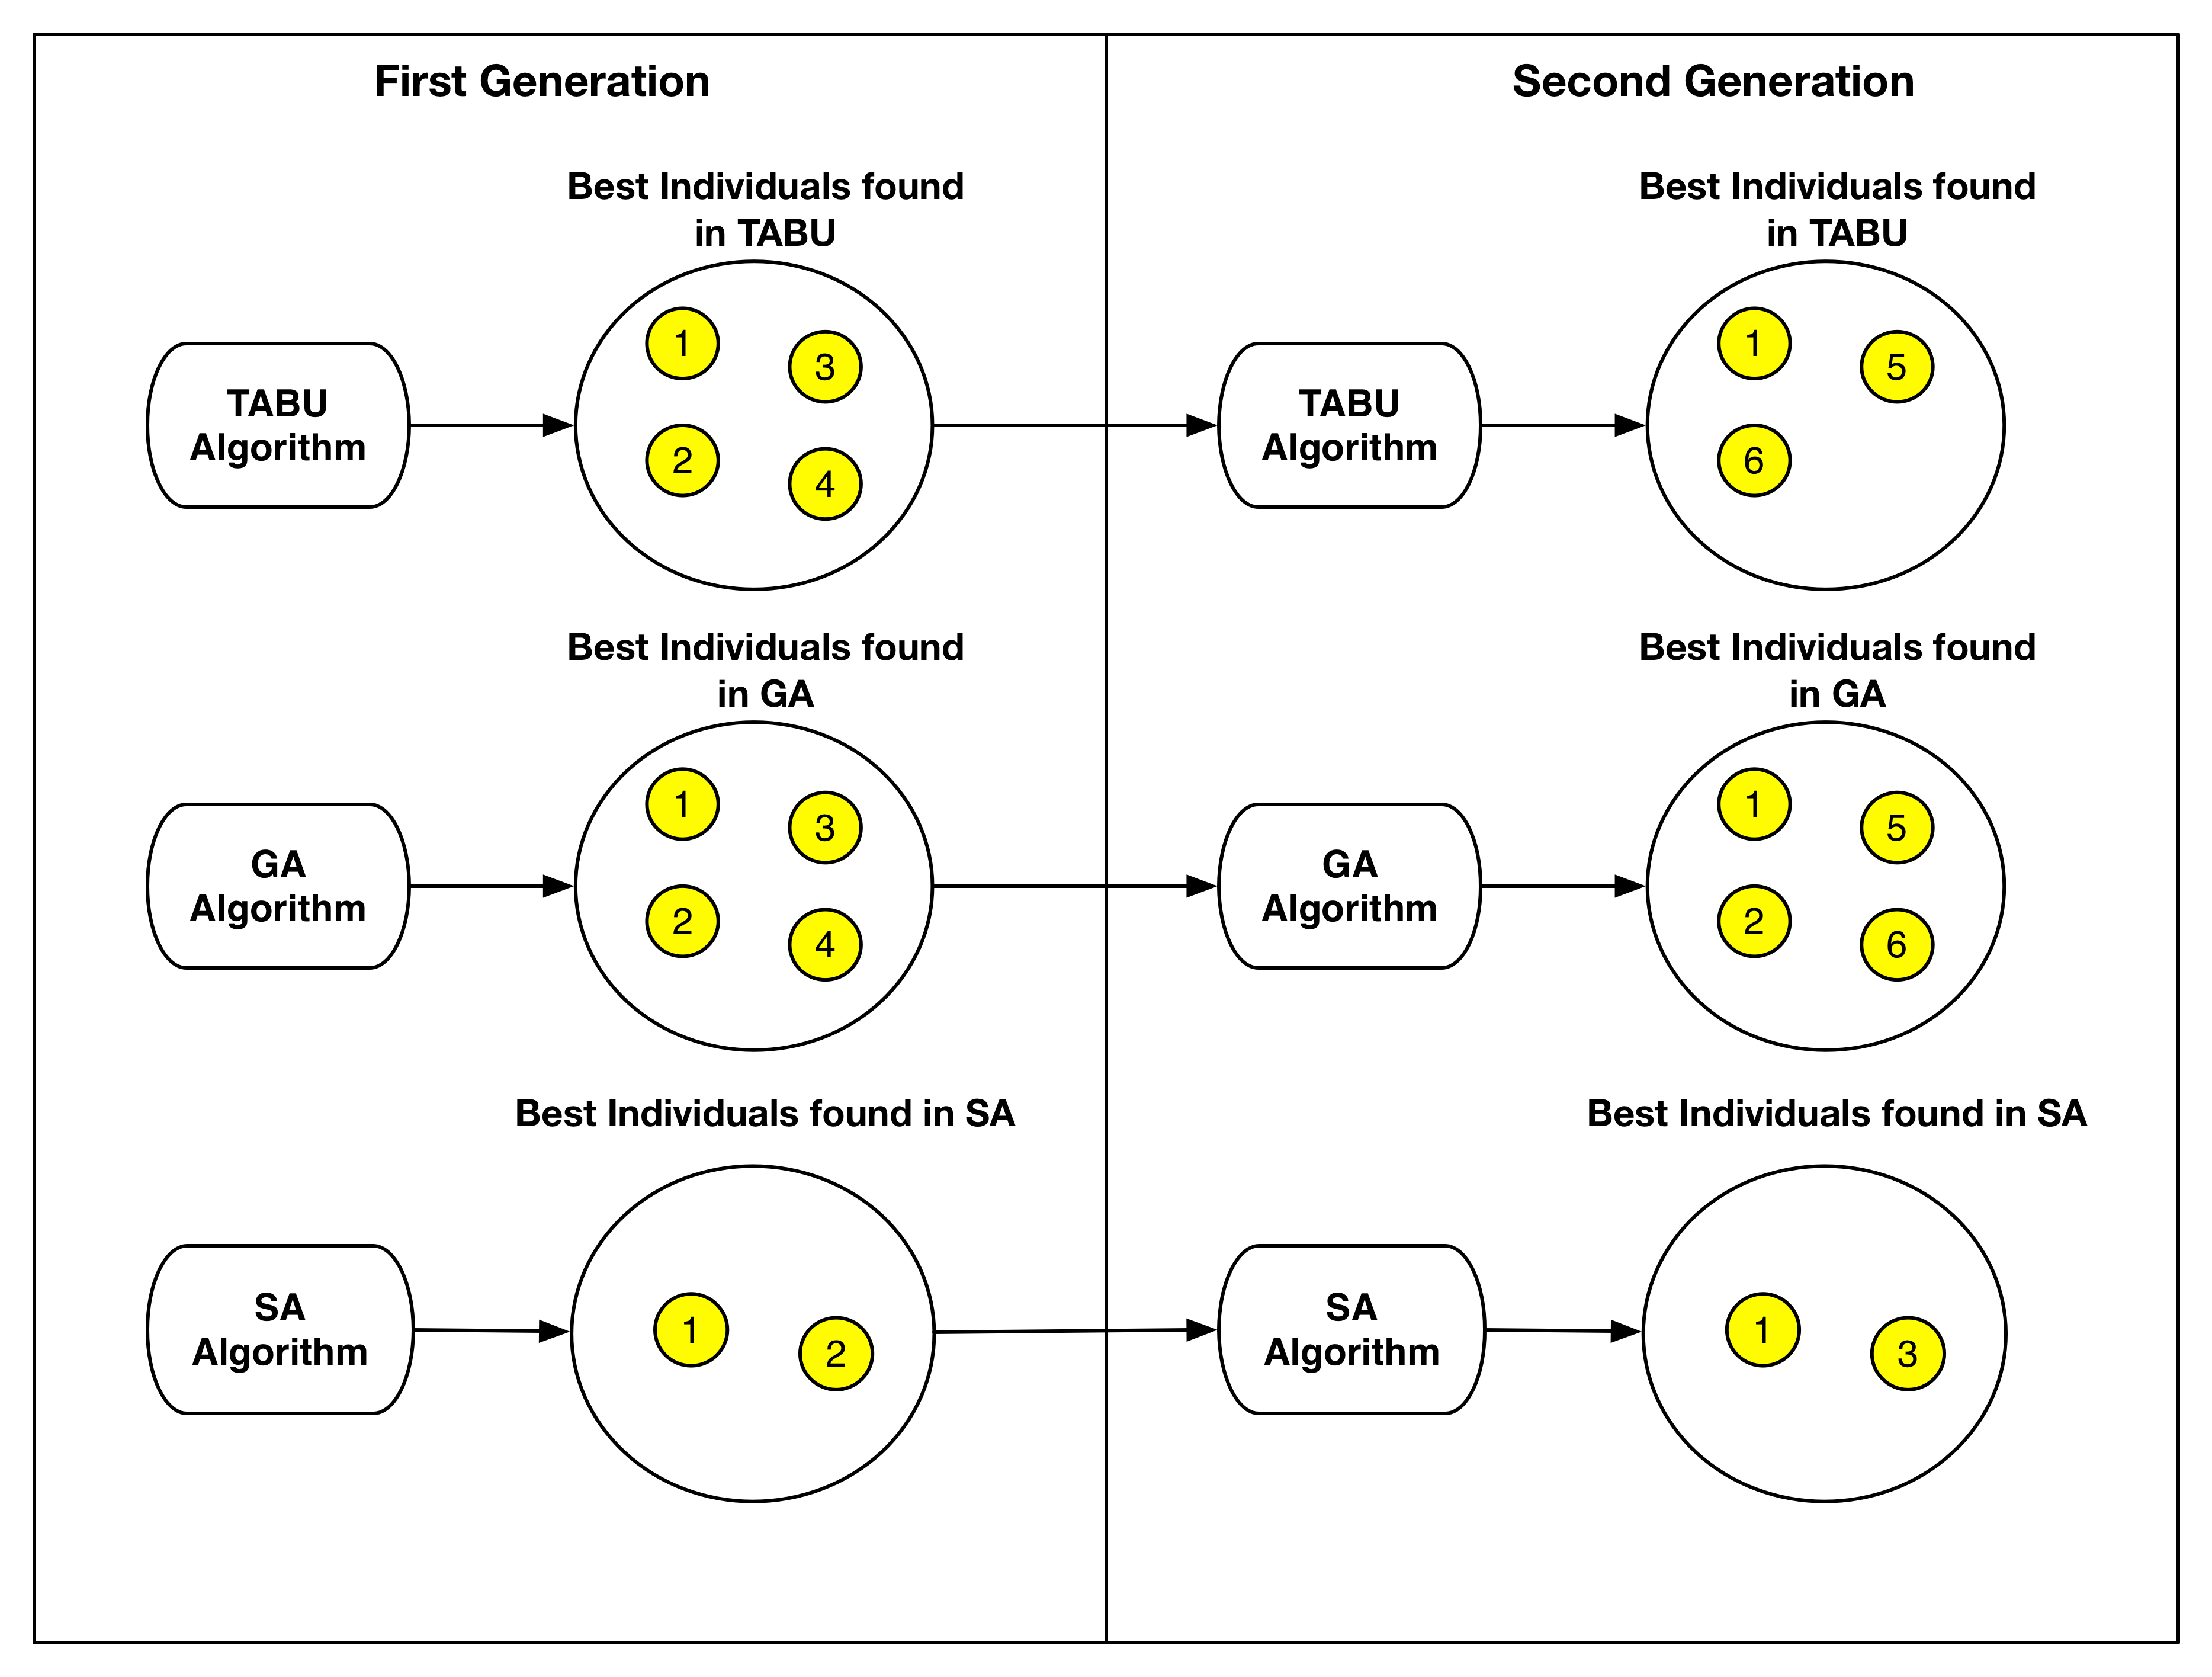
\includegraphics[width=0.5\textwidth]{./images/independ.png}
\caption{Use of the algorithms independently}
\label{fig:firstaproach}
\end{figure}
\begin{figure}
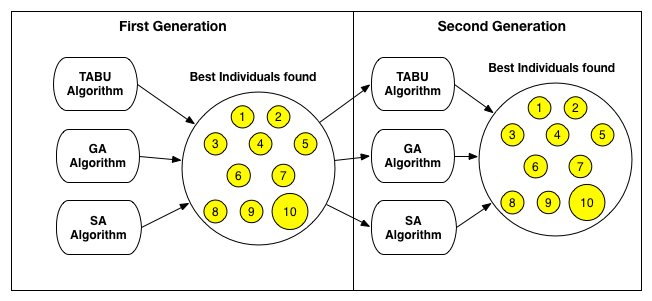
\includegraphics[width=0.5\textwidth]{./images/collaborative.png}
\caption{Use of the  algorithms collaboratively}
\label{fig:secondapproach}
\end{figure}

\subsection{Genotype representation}

The genotype representation is composed by a linear vector with 23 genes. The first gene represents the name of an individual. The second gene represents the algorithm (genetic algorithm, simulated annealing, or Tabu search) used by the individual. The third gene represents the type of test (load, stress, or performance). The next genes represent 10 scenarios and their numbers of users. Each scenario is an atomic operation: the scenario must log into the application, run the task goal, and undo any changes performed, returning the application to its original state.

Fig. \ref{fig:genomarepresentation} presents the genome representation and an example using the crossover operation. In the example, genotype 1 has the Login scenario with 2 users, the Form scenario with 0 users, and the Search scenario with 3 users. Genotype 2 has the Delete scenario with 10 users, the Search scenario with 0 users, and the Include scenario with 5 users. After the crossover operation, we obtain a genotype with the Login scenario with 2 users, the Search scenario with 0 users, and the Include scenario with 5 users.

\begin{figure}[h]
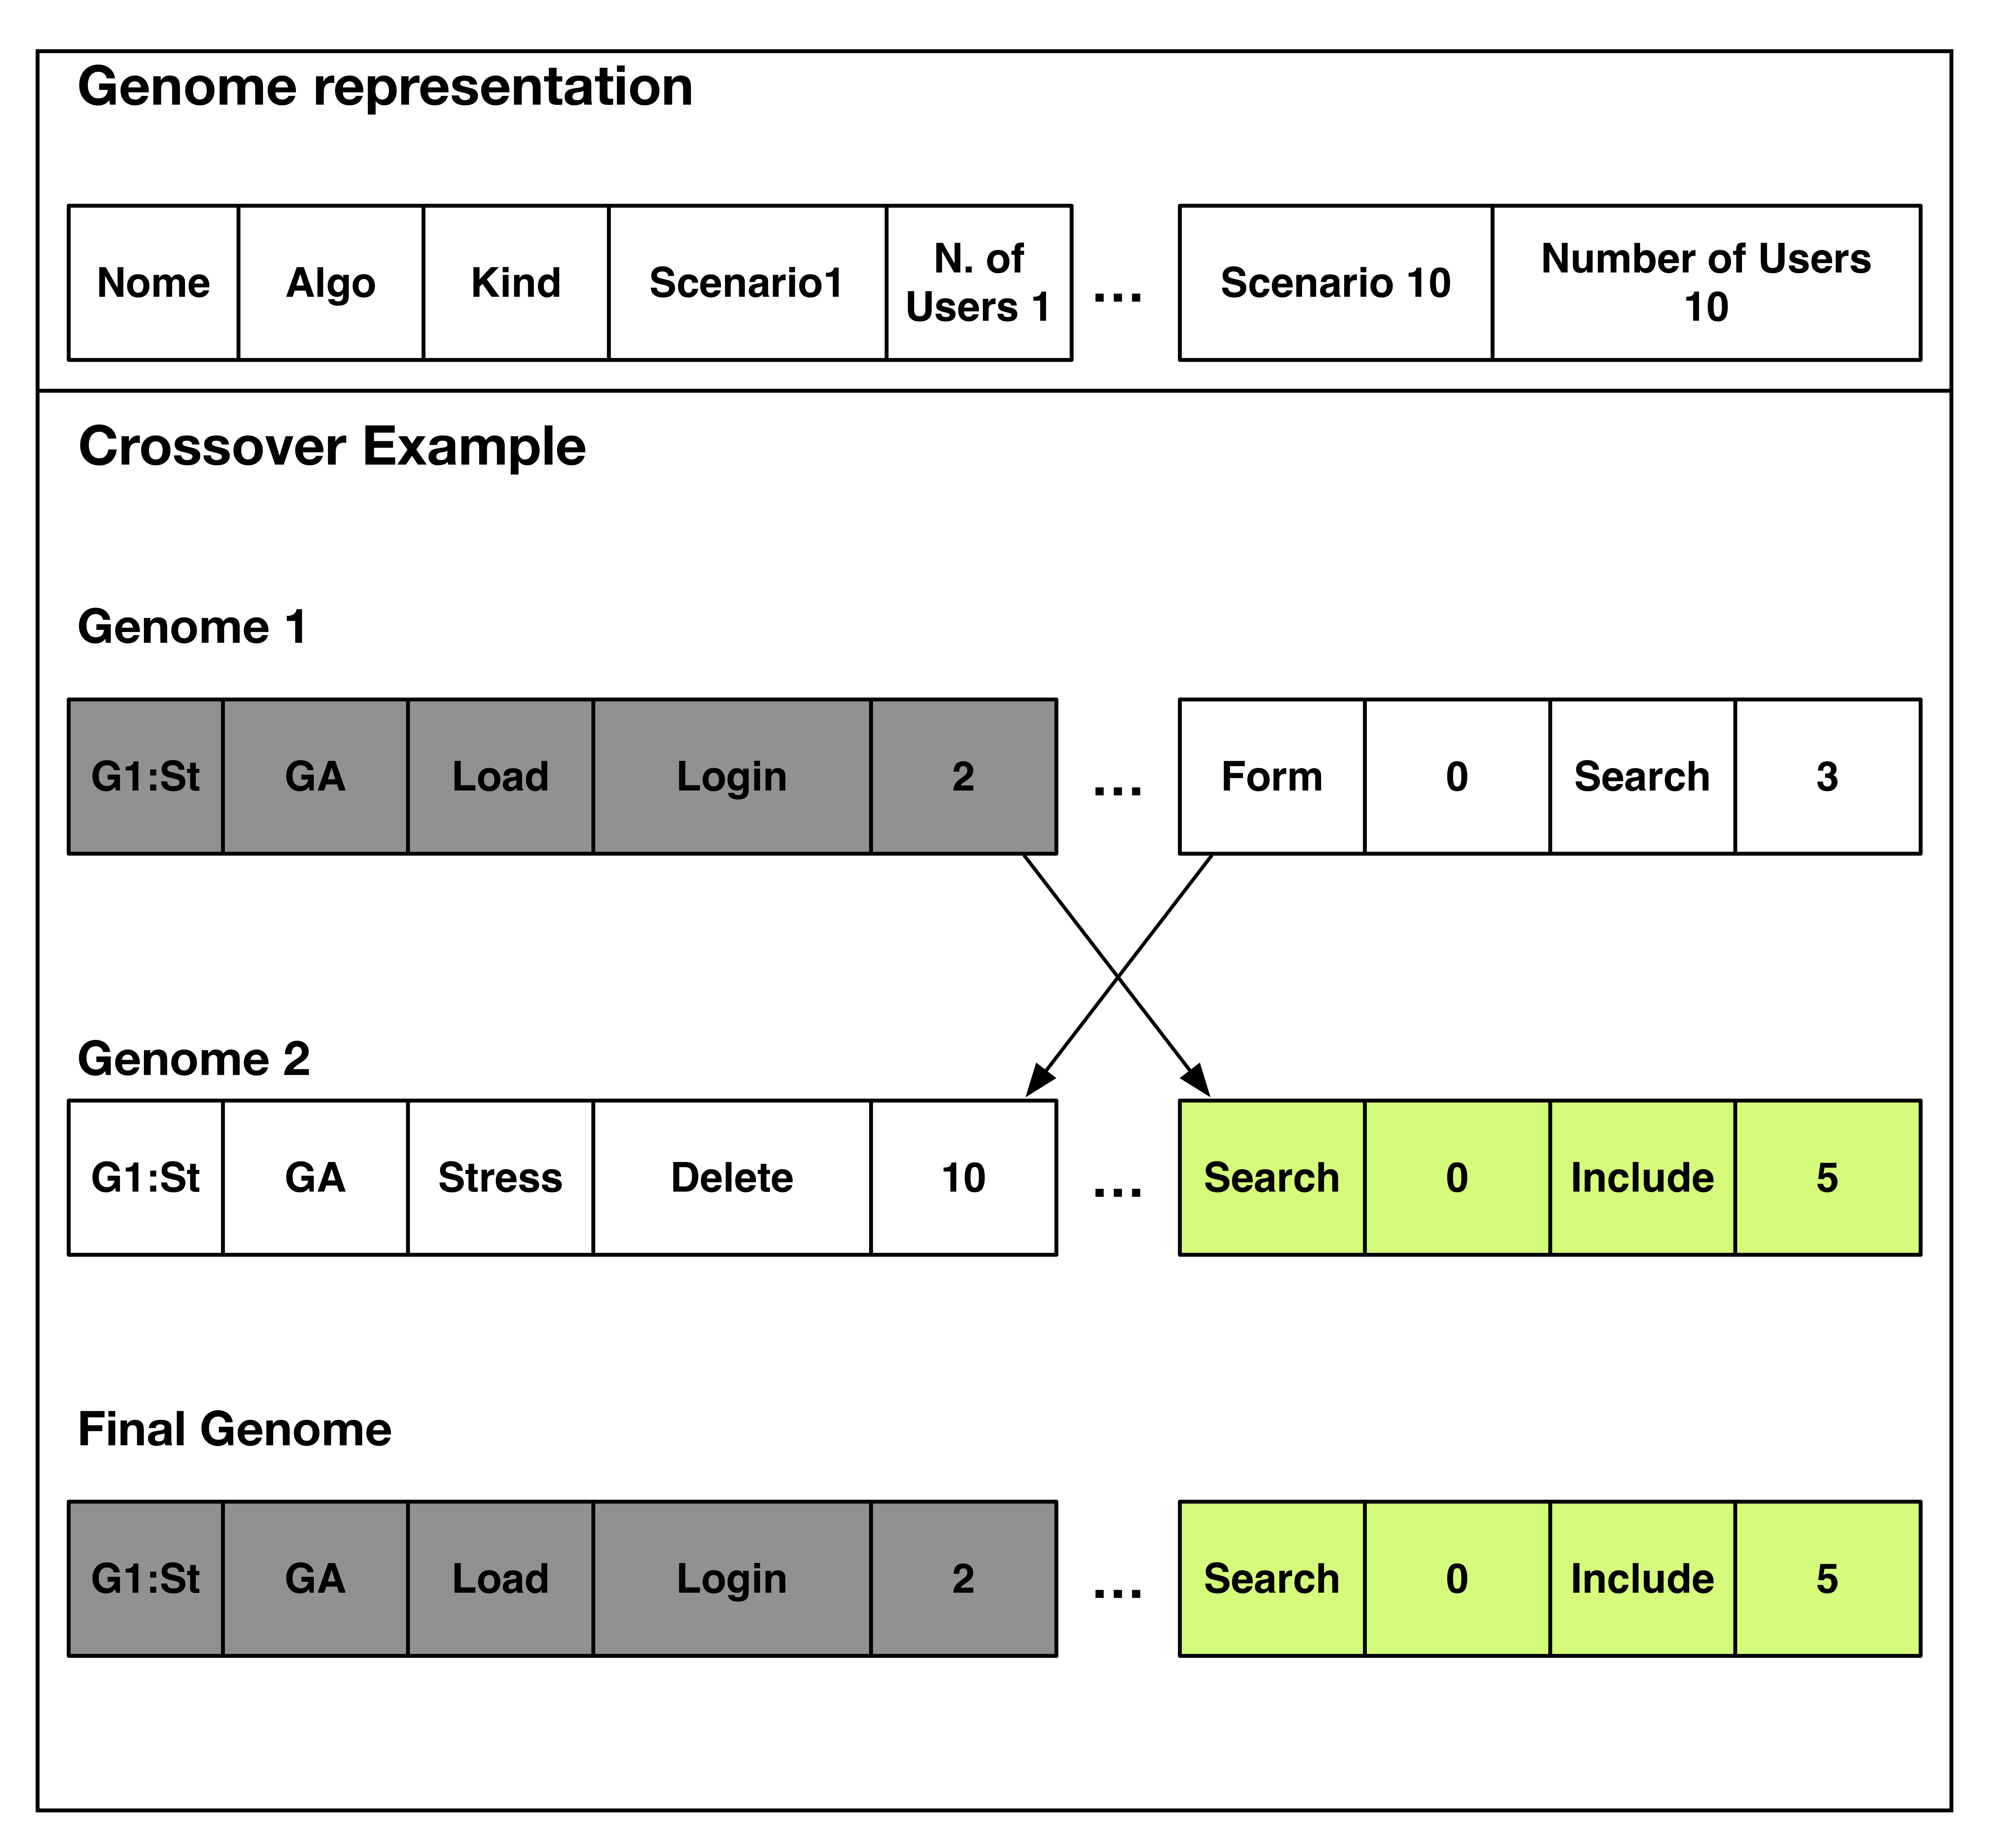
\includegraphics[width=0.5\textwidth]{./images/genomerepresentation.png}
\caption{Genotype representation and crossover example}
\label{fig:genomarepresentation}
\end{figure}

Fig. \ref{fig:neighbourtaby} shows the strategy used by the IAdapter tool to obtain the genotype of the neighbors for the Tabu search and simulated annealing algorithms. The neighbors are obtained by the modification of a single chromosome (scenario or number of users) in the genotype.


\begin{figure}[h]
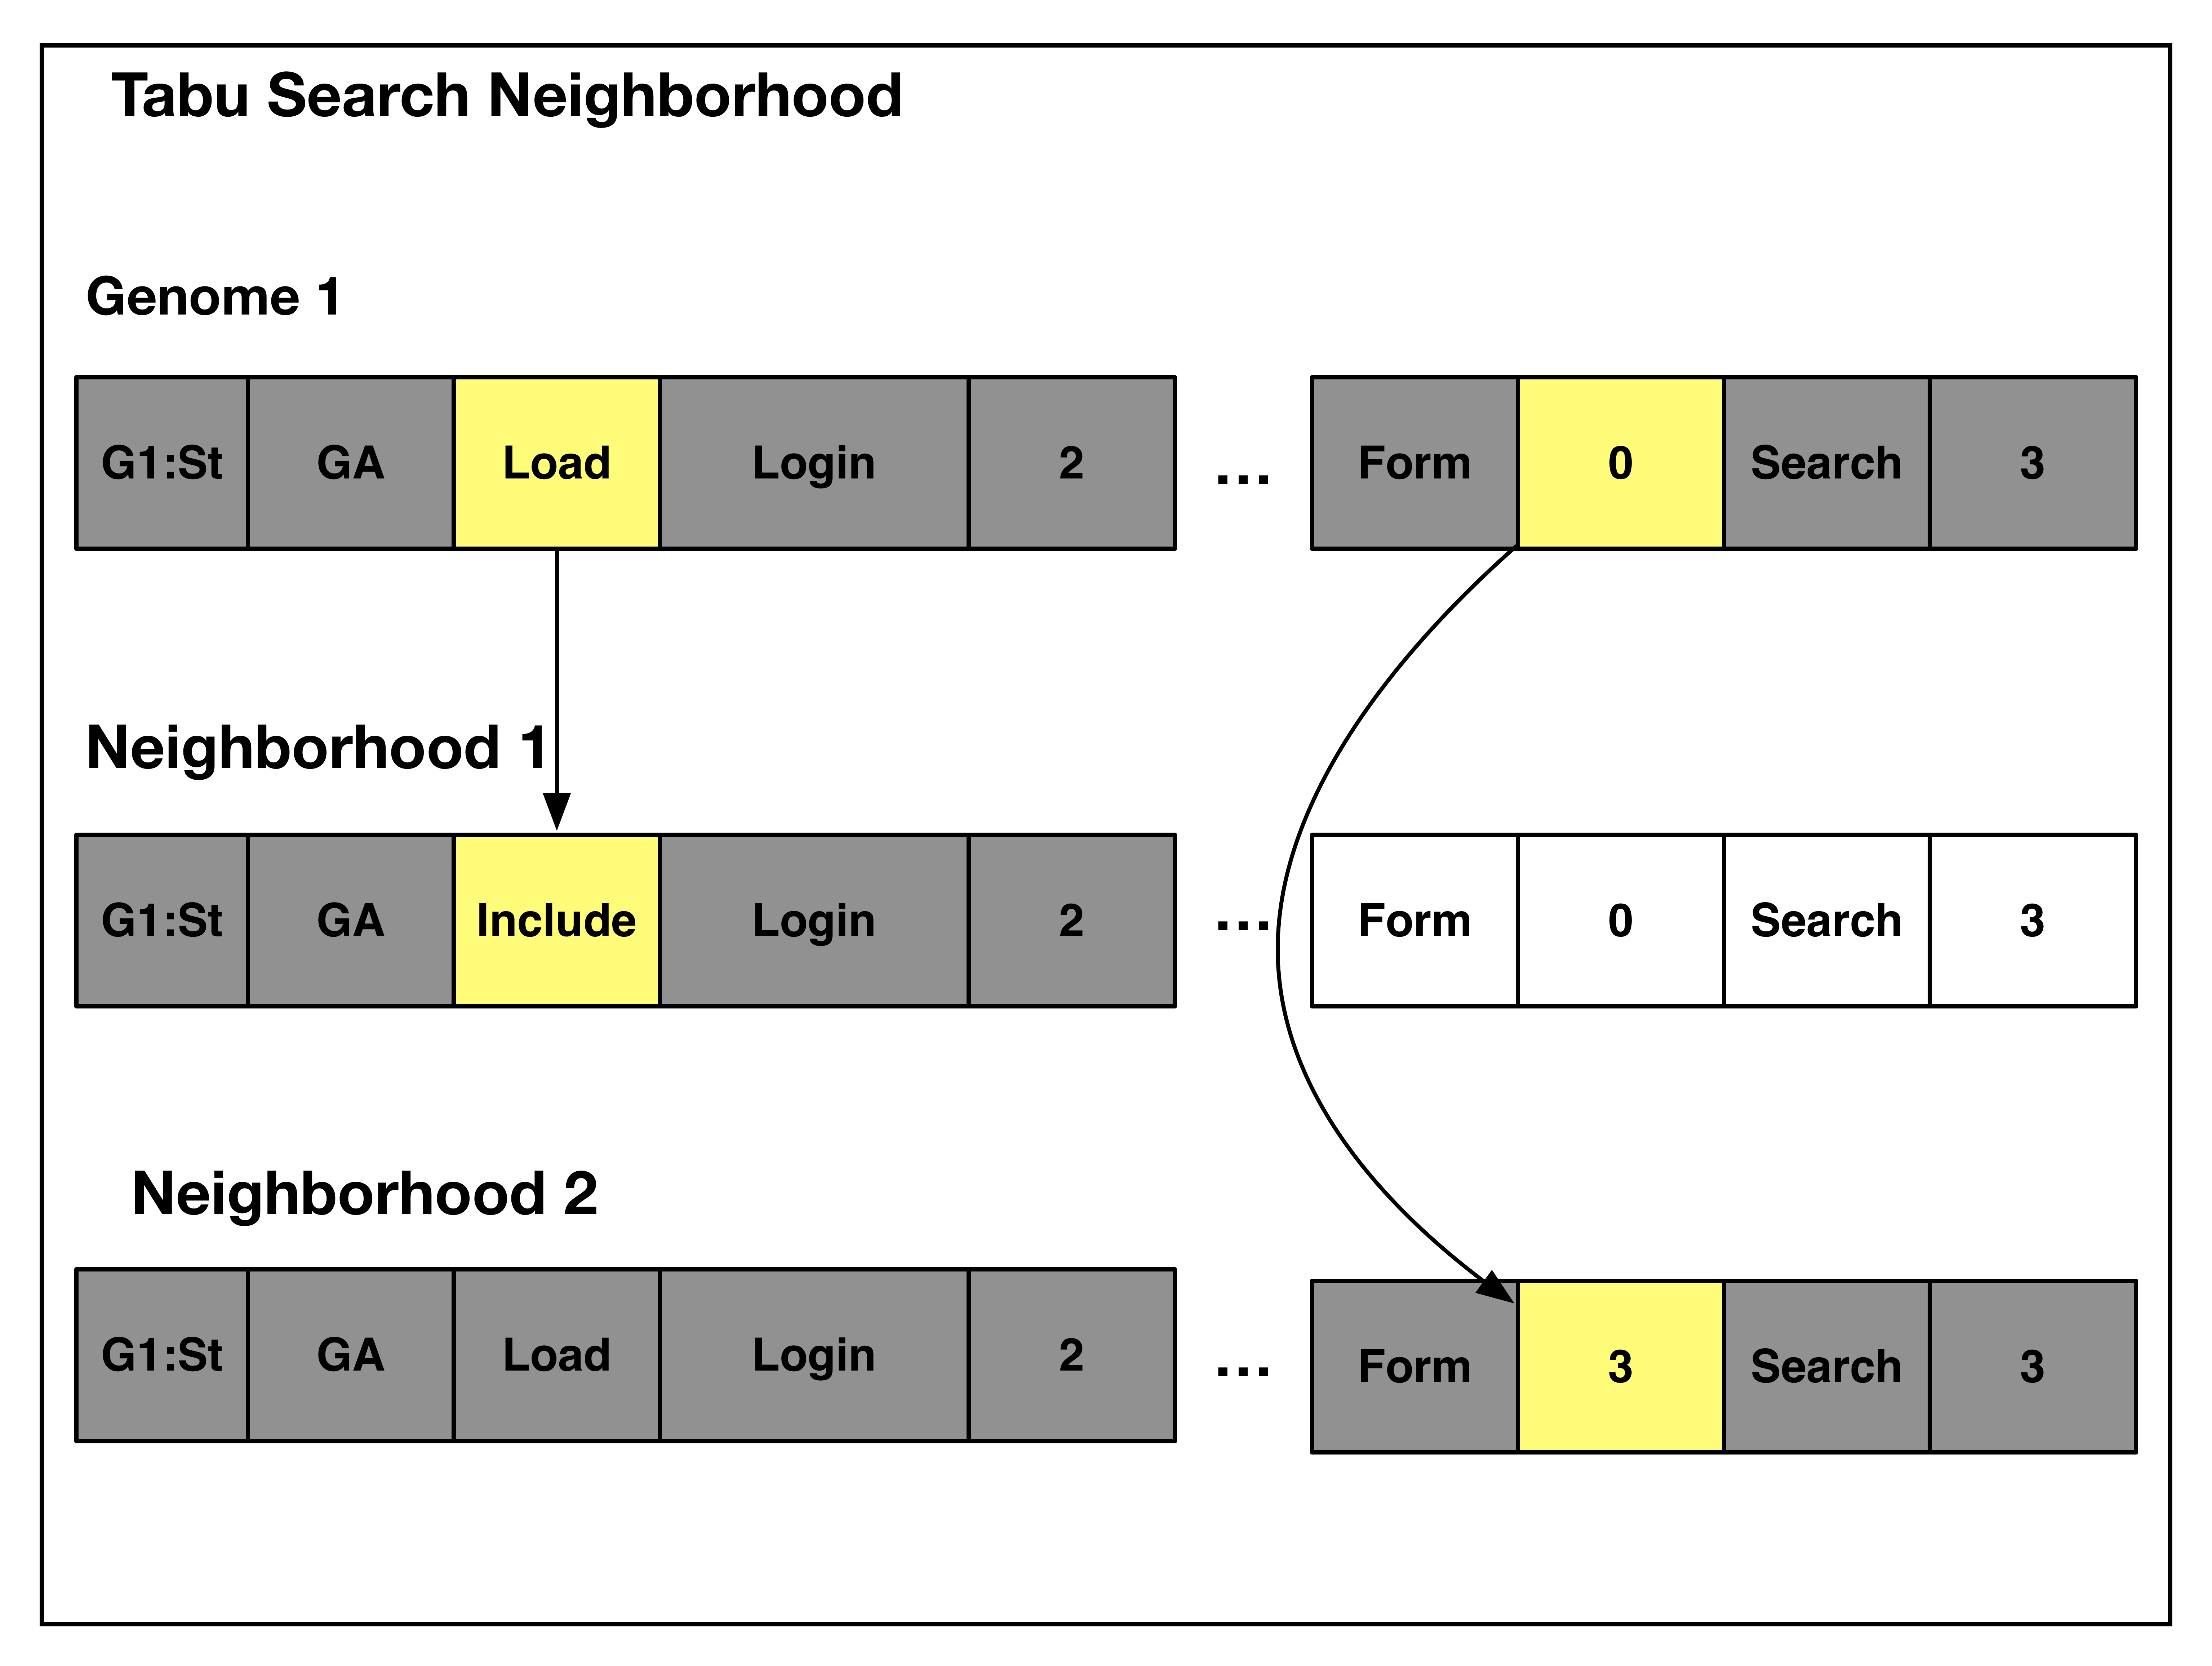
\includegraphics[width=0.5\textwidth]{./images/TabuNE.png}
\caption{Tabu search and simulated annealing neighbor strategy}
\label{fig:neighbourtaby}
\end{figure}


\subsection{Initial population}

The strategy used by the plugin to instantiate the initial population is to generate 50\% of the individuals randomly, and 50\% of the initial population is distributed in three ranges of values:

\begin{itemize}
\item Thirty percent of the maximum allowed users in the test;
\item Sixty percent of the maximum allowed users in the test; and
\item Ninety percent of the maximum allowed users in the test.
\end{itemize}

\subsection{Objective (fitness) function}

The proposed solution was designed to be used with independent testing teams in various situations where the teams have no direct access to the environment where the application under test was installed. Therefore, the IAdapter plugin uses a measurement approach to the definition of the fitness function. The fitness function applied to the IAdapter solution is governed by the following equation:

\begin{equation}
\begin{aligned}
fit=90percentileweigth* 90percentiletime\\
+80percentileweigth*80percentiletime\\+
70percentileweigth*70percentiletime+\\
maxResponseWeigth*maxResponseTime+\\
numberOfUsersWeigth*numberOfUsers-penalty
\end{aligned}
\end{equation}

The proposed solution's fitness function uses a series of adaptable user-defined weights (90percentileweight, 80percentileweight,  70percentileweight, maxResponseWeight, and numberOfUsersWeight). These weights make it possible to customize the search plugin's functionality. A penalty is applied when an application under test takes a longer time to respond than the level of service.


%\FloatBarrier
\section{IAdapter}

IAdapter is a JMeter plugin designed to perform search-based load, performance, or stress tests. JMeter is a desktop application designed to test and measure the performance and functional behavior of applications \cite{Nevedrov2007}. The IAdapter plugin implements the solution proposed in Section 6.

JMeter has components organized  in a hierarchical manner. The IAdapter plugin provides three main components: WorkLoadThreadGroup, WorkLoadSaver, and WorkLoadController.
 
WorkLoadThreadGroup is a component that creates an initial population and configures the algorithms used in IAdapter. Fig. \ref{fig:tela1iadapter} presents the main screen of the WorkLoadThreadGroup component. The component has a name \ding{202}, a set of configuration tabs \ding{203}, a list of individuals by generation \ding{204}, a button to generate an initial population \ding{205}, and a button to export the results \ding{206}.

\begin{figure}[h]
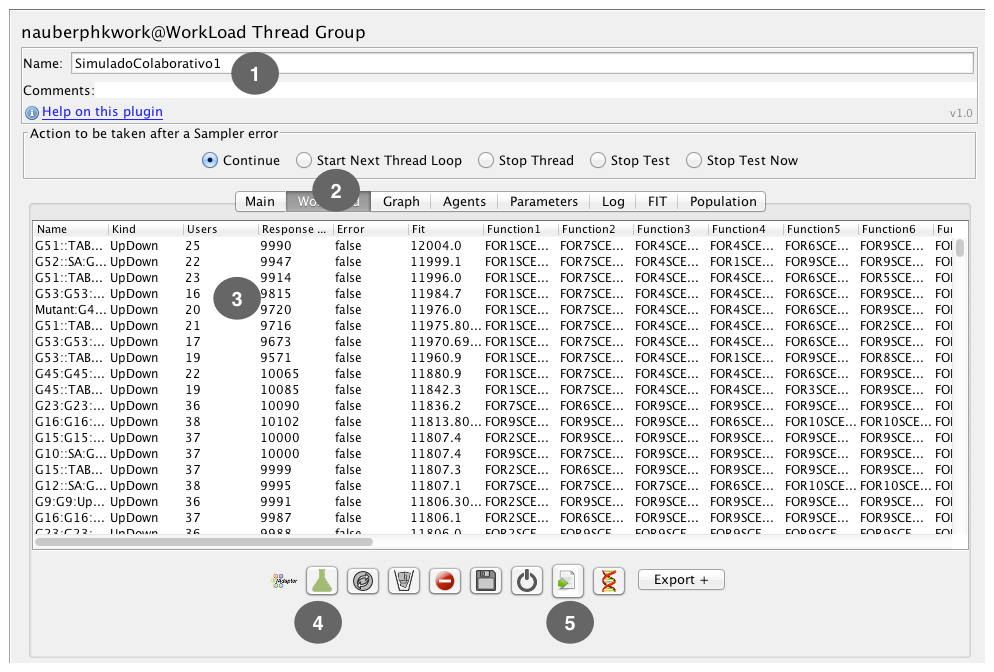
\includegraphics[width=0.5\textwidth]{./images/tela1iadapter.png}
\caption{WorkLoadThreadGroup component}
\label{fig:tela1iadapter}
\end{figure}

The WorkLoadSaver component is responsible for saving all data in the database. The operation of the component only requires its inclusion in the test script.

WorkLoadController represents a scenario of the test. All actions necessary to test an application should be included in this component. All instances of the component need to login to the application under test and return the application to its original state.

\section{Related Work}

The search for the longest execution time is regarded as a discontinuous, nonlinear, optimization problem, with the input domain of the system under test as a search space \cite{Sullivan}. The main objective of search-based testing in performance, stress, and load tests is to find test scenarios that produce execution times that exceed the timing constraints specified. If a temporal error is found, the test was successful \cite{Sullivan}. The application of evolutionary algorithms to load, performance, and stress tests involves finding the best- and worst-case execution times to determine whether timing constraints are fulfilled \cite{Afzal2009a}. 

Some search-based tests use a cost (fitness) function to select the best individuals. There are two measurement units normally associated with the fitness function in a load, performance, or stress test: processor cycles and execution time. The processor cycle approach describes a fitness function in terms of processor cycles. The execution time approach involves executing the application under test and measuring the execution time \cite{Afzal2009} \cite{tracey2000search}.

Table \ref{tab:comparison}  shows a comparison between the presented research work and the research studies on load, performance, and stress tests presented by Afzal et al. \cite{Afzal2009}. Afzal's work adds to some of the latest research in this area (\cite{Garousi2006} \cite{Garousi2010} \cite{DiAlesio2013} \cite{DiAlesio2014} \cite{Alesio2015}). 


The columns represent the type of tool used (prototype or functional tool), and the rows represent the metaheuristic approach used by each research study (genetic algorithm, Tabu search, simulated annealing, or a customized algorithm). The table also divides the research studies by the type of fitness function used (execution time or processor cycles). Most research studies are limited to making prototypes of genetic algorithms. The presented research work is distinguished from others by having a functional tool using a hybrid approach. 





% * <naubergois@gmail.com> 2015-09-17T01:22:09.554Z:
%
%  Customized Algorithm
%

%\begin{figure}[h]
%\centering
%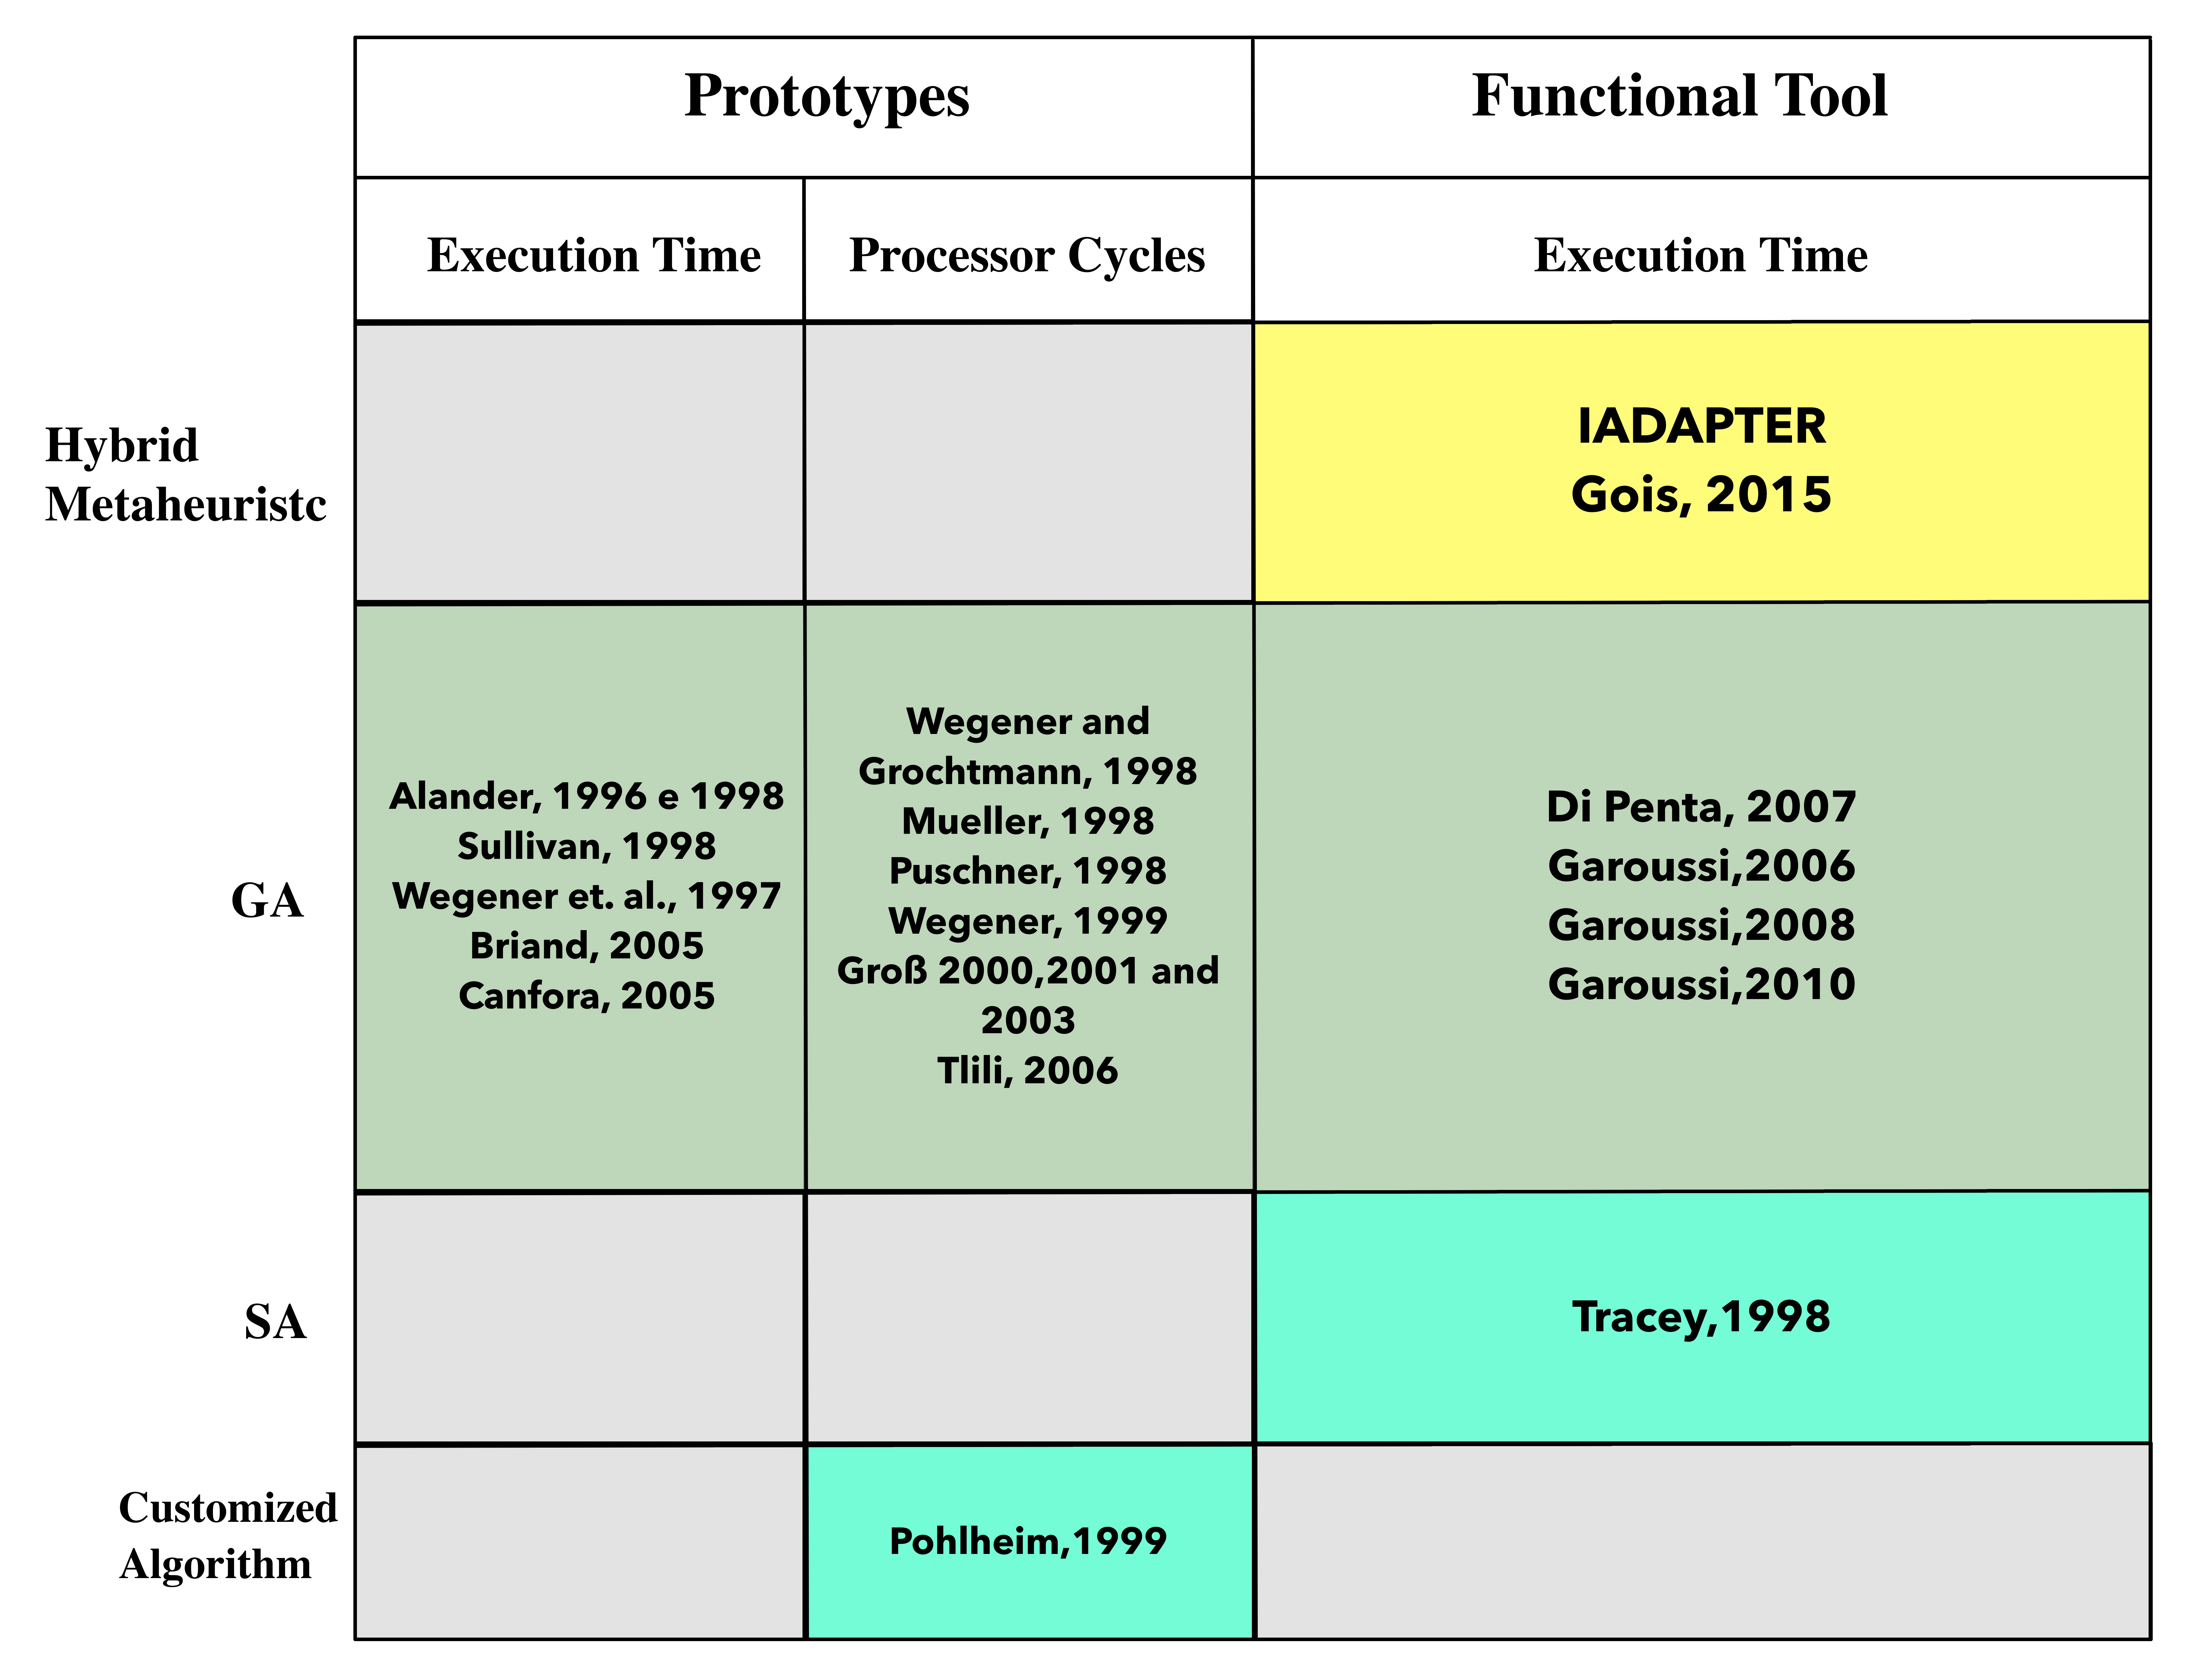
\includegraphics[width=0.5\textwidth]{./images/comparativo1.png}
%\caption{
%Distribution of the researches over range of applied metaheuristics}
%\label{fig:comparison}
%\end{figure}

% Please add the following required packages to your document preamble:
% \usepackage[table,xcdraw]{xcolor}
% If you use beamer only pass "xcolor=table" option, i.e. \documentclass[xcolor=table]{beamer}
\begin{table}[h]
\centering
\caption{Distribution of the research studies over the range of applied metaheuristics}
\label{tab:comparison}
\begin{tabular}{p{1.2cm}|p{1.8cm}|p{1.8cm}|p{1.8cm}|}
\cline{2-4}
                                                                & \multicolumn{2}{c|}{\textbf{Prototypes}}            & \textbf{Functional Tool} \\ \cline{2-4} 
                                                                & \begin{minipage}{0.2\textwidth}\footnotesize Execution Time  \end{minipage}          & \begin{minipage}{0.2\textwidth}\footnotesize Processor Cycles \end{minipage}        & \begin{minipage}{0.2\textwidth}\footnotesize Execution Time \end{minipage}           \\ \cline{2-4} 
%\setlength{\extrarowheight}{20pt}
\begin{tabular}[c]{@{}l@{}}\begin{minipage}{0.1\textwidth}\scriptsize GA + SA  \\ + Tabu \\ Search \end{minipage}\end{tabular}  & \cellcolor[HTML]{FFCCC9} & \cellcolor[HTML]{FFCCC9} & \cellcolor[HTML]{F8FF00} \begin{minipage}{0.2\textwidth} \scriptsize \textbf{  \\ IADAPTER \\ Gois, 2015 \\} \end{minipage}  \\[2ex] \cline{2-4} 
\begin{minipage}{0.1\textwidth}\scriptsize GA \end{minipage}                                                              & \cellcolor[HTML]{CD9934} \begin{minipage}{0.12\textwidth}   \tiny \textnormal{ \\  Alander et al.,1998 \cite{Alander} \\ Wegener et al., 1996 and 1997 \cite{Wegener1997}\cite{J.WegenerK.GrimmM.GrochtmannH.Sthamer1996} \\  Sullivan et al., 1998 \cite{Sullivan} \\ Briand et al., 2005 \cite{Briand2005} \\ Canfora et al., 2005 \cite{Canfora}  \\ }\end{minipage} & \cellcolor[HTML]{CD9934} \begin{minipage}{0.12\textwidth} \tiny \textrm{  \\ Wegener and Grochtmann, 1998 \cite{Wegener1998} \\  Mueller et al., 1998 \cite{Mueller1998} \\ Puschner et al. \cite{Puschner1998} \\ Wegener et al., 2000 \cite{Stations} \\ Gro et al., 2000 \cite{Gross2000}  \\ }\end{minipage}& \cellcolor[HTML]{CD9934} \begin{minipage}{0.12\textwidth}   \tiny \textnormal{ \\  Di Penta, 2007 \cite{Penta2007} \\ Garoussi, 2006 \cite{Garousi2006} \\ Garousi, 2008 \cite{Garousi2008} \\ Garousi, 2010 \cite{Garousi2010} \\ } \end{minipage} \\[2ex] \cline{2-4} 
\begin{minipage}{0.1\textwidth}\scriptsize Simulated \\ Annealing \\ (SA) \end{minipage}                                                             & \cellcolor[HTML]{FFCCC9} & \cellcolor[HTML]{FFCCC9} & \cellcolor[HTML]{CD9934} \begin{minipage}{0.12\textwidth}   \tiny  Tracey, 1998 \cite{Tracey1998} \end{minipage} \\[2ex] \cline{2-4}
\begin{minipage}{0.1\textwidth}\scriptsize  Constraint \\ Programming \end{minipage}                                                             & \cellcolor[HTML]{FFCCC9} & \cellcolor[HTML]{FFCCC9} & \cellcolor[HTML]{CD9934} \begin{minipage}{0.12\textwidth}   \tiny  Alesio, 2014 \cite{DiAlesio2014} \\ Alesio, 2013 \cite{DiAlesio2013}  \end{minipage} \\[2ex] \cline{2-4} 
\begin{minipage}{0.1\textwidth}\scriptsize  GA +\\ Constraint \\ Programming \end{minipage}                                                             & \cellcolor[HTML]{FFCCC9} & \cellcolor[HTML]{FFCCC9} & \cellcolor[HTML]{CD9934} \begin{minipage}{0.12\textwidth}   \tiny  Alesio, 2015 \cite{Alesio2015} \end{minipage} \\[2ex] \cline{2-4} 
\setlength{\extrarowheight}{20pt}
\begin{tabular}[c]{@{}l@{}}
\begin{minipage}{0.1\textwidth}\scriptsize Customized \\ Algorithm \end{minipage}\end{tabular} & \cellcolor[HTML]{FFCCC9} & \cellcolor[HTML]{CD9934}  \begin{minipage}{0.12\textwidth}   \tiny  \textnormal{   \raggedleft Pohlheim, 1999 \cite{Pohlheim2005}  } \end{minipage} & \cellcolor[HTML]{FFCCC9} \\[4ex] \cline{2-4}
\end{tabular}
%\begin{tabular}[c]{@{}l@{}}
%\begin{minipage}{0.1\textwidth}\scriptsize GA  Constraint Programming \end{minipage}\end{tabular} & \cellcolor[HTML]{FFCCC9} & \cellcolor[HTML]{CD9934}  \begin{minipage}{0.12\textwidth}   \tiny  \textnormal{   \raggedleft Alesio, 2015 \cite{Alesio2015}   } \end{minipage} & \cellcolor[HTML]{FFCCC9} \\[4ex] \cline{2-4}
%\end{tabular}
\end{table}

The presented research work and Alesio's approach \cite{Alesio2015} use a hybrid approach with a functional tool. Table \ref{tab:alesiogois} presents the main differences between Alesio's and Gois's approaches. Whereas the present research uses an approach based on usage scenarios performing tests on an application installed in an available environment, Alesio uses sequence diagrams  to select for arrival time of tasks in systems from  safety-critical domains. 


\begin{table}[h]
\centering
\caption{Main differences between Alesio's \cite{Alesio2015} and Gois's approaches}
\label{tab:alesiogois}
\begin{tabular}{l|l|l|}
\cline{2-3}
                                                                                  & Alesio et al. \cite{Alesio2015}                                                                                                             & Gois et al.                                                                                                                            \\ \hline
\multicolumn{1}{|l|}{Metaheuristcs}                                               & \begin{tabular}[c]{@{}l@{}}GA+ \\ Constraint Programming\end{tabular}                                                      & \begin{tabular}[c]{@{}l@{}}GA+SA+\\ Tabu Search\end{tabular}                                                                           \\ \hline
\multicolumn{1}{|l|}{Inputs}                                                      & \begin{tabular}[c]{@{}l@{}}Design Model (Time and \\ Concurrency\\  Information)\end{tabular}                              & \begin{tabular}[c]{@{}l@{}}Number of Users\\ Ramp-up\\ Test scenarios\end{tabular}                                                     \\ \hline
\multicolumn{1}{|l|}{\begin{tabular}[c]{@{}l@{}}Main\\ Objective\end{tabular}}    & \begin{tabular}[c]{@{}l@{}}Find task arrival times\\ of aperiodic tasks that\\  maximizing\\  deadline misses\end{tabular} & \begin{tabular}[c]{@{}l@{}}Find the number of\\  users, ramp-up and \\ test scenarios that\\ maximizing\\ deadline misses\end{tabular} \\ \hline
\multicolumn{1}{|l|}{\begin{tabular}[c]{@{}l@{}}Main \\ Application\end{tabular}} & \begin{tabular}[c]{@{}l@{}}Systems from \\ safety-critical \\ domains\end{tabular}                                         & \begin{tabular}[c]{@{}l@{}}Web and Mobile \\ applications\end{tabular}                                                                 \\ \hline
\end{tabular}
\end{table}



%\nocite{Alander,Sullivan,Wegener1997,Briand2005,Canfora,Wegener1998,Mueller1998,Puschner1998,Wegener1999,Gro,Gross2003,Tlili1917}


\section{Experiments}

This section presents two experiments. The first one was performed on an emulated component, and the second one was performed using an installed Moodle application. The experiments used the following fitness function:

\begin{equation}
\begin{aligned}
fit=0.9* 90percentiletime\\
+0.1*80percentiletime\\+
0.1*70percentiletime+\\
0.1*maxResponseTime+\\
0.2*numberOfUsers-penalty
\end{aligned}
\end{equation}

This fitness function intended to find individuals with the highest percentile of 90\%, followed by individuals with a higher percentile time of 80\% and 70\%, maximum response time, and number of users.

The first experiment implemented 27 generations, and the second experiment  performed 6 generations, with 300 executions by generation (100 times for each algorithm),  generating 300 new individuals. The experiments used an initial population of 100 individuals. The genetic algorithm used the top 10 individuals from each generation in the crossover operation. The Tabu list was configured with the size of 10 individuals and expired every 2 generations.  The mutation operation was applied to 10\% of the population on each generation. 

\subsection{First Experiment: Emulated Class Test}

The first experiment aimed to perform performance, load, and stress testing on a simulated component. The purpose of using a simulated component was to be able to perform a greater number of generations in a shorter time available and eliminate variables such as the use of databases and application servers. The first experiment used a test class  named SimulateConcurrentAccess. This class has a static variable named \textit{x} and a set of methods that use the variable in a synchronized context ( Listing \ref{classsimulated}).


\lstdefinestyle{outline}{
		language=Java,
         basicstyle=\scriptsize\ttfamily,
         numberstyle=\tiny,
         numbersep=5pt,
         tabsize=2,
         extendedchars=true,
         breaklines=true,
         keywordstyle=\color{black}\bf,
         frame=b,  % <<<<<<<<<<<<<<<<<<<<<<<<<<
         stringstyle=\color{green!40!black}\ttfamily,
         showspaces=false,
         showtabs=false,
         numbers=left,
         xleftmargin=17pt,
         framexleftmargin=17pt,
         framextopmargin=1pt, % <<<<<<<<<<<<<<<<<<<<<<
         showstringspaces=false,
         %backgroundcolor=\color[RGB]{200,200,200},
         belowcaptionskip=0pt
}

\begin{lstlisting}[style=outline,caption={SimulateConcurrentAcess class},float,label=classsimulated]
public class SimulateConcurrentAccess {
  @Test
  public void firstScenario() {		
    synchronized (StaticClass.class) {
			for (int i = 0; i <= 1000; i++) {
				StaticClass.x += i;
			}
			StaticClass.x = 0;
		}
	}
	
	  @Test
  public void secondScenario() {		
    synchronized (StaticClass.class) {
			for (int i = 0; i <= 2000; i++) {
				StaticClass.x += i;
			}
			StaticClass.x = 0;
		}
	}
\end{lstlisting}


Fig.\ref{fig:exp1bestresults} presents the best results in 27 generations applied in the first experiment. The figure shows the results obtained with the algorithms with and without collaboration. The $x$ axis  represents the generation number, and the $y$ axis represents the best fitness value obtained until the current generation. The results of the experiment showed that the use of cooperation between the three algorithms resulted in finding the individuals with better fitness values.

\begin{figure}[h]
\centering
\caption{Best results obtained in 27 generations}
\includegraphics[width=0.5\textwidth]{./images/generationcomparative.png}
\label{fig:exp1bestresults}
\end{figure}

Table \ref{tab:averagefirst} presents the results obtained by the hybrid metaheuristic (HM) approach, genetic algorithm (GA), simulated annealing (SA), and Tabu search (TS) from 27 generations in the first experiment. The values are the maximum value of the fitness value obtained in each algorithm. 

\begin{table}[h]
\centering
\caption{Maximum value of the fitness function by algorithm}
\label{tab:averagefirst}
\begin{tabular}{|l|l|l|l|l|}
\hline
GEN & HM & TS  & GA    & SA    \\ \hline
1          & 11238 & 11238         & 11238 & 11238 \\ \hline
2          & 11804 & 11596         & 11801 & 10677 \\ \hline
3          & 11787 & 8932          & 8411  & 10869 \\ \hline
4          & 11723 & 9753          & 9611  & 10760 \\ \hline
5          & 8164  & 9780          & 10738 & 4794  \\ \hline
6          & 11802 & 9781          & 11086 & 6120  \\ \hline
7          & 9985  & 5782          & 11272 & 11798 \\ \hline
8          & 11803 & 11749         & 10084 & 11309 \\ \hline
9          & 11806 & 7284          & 11633 & 10766 \\ \hline
10         & 11807 & 9386          & 11717 & 4557  \\ \hline
11         & 11802 & 9653          & 11802 & 11151 \\ \hline
12         & 11807 & 10594         & 11793 & 9434  \\ \hline
13         & 11802 & 10848         & 10382 & 11805 \\ \hline
14         & 11801 & 11551         & 7219  & 10237 \\ \hline
15         & 11807 & 1701          & 7189  & 9338  \\ \hline
16         & 11813 & 6203          & 11758 & 5321  \\ \hline
17         & 11805 & 10720         & 10805 & 11748 \\ \hline
18         & 9600  & 6371          & 11698 & 7818  \\ \hline
19         & 11733 & 8160          & 11648 & 11509 \\ \hline
20         & 9589  & 9428          & 11805 & 4813  \\ \hline
21         & 11800 & 9463          & 11798 & 10801 \\ \hline
22         & 11805 & 11799         & 11804 & 6029  \\ \hline
23         & 11836 & 11655         & 11800 & 3579  \\ \hline
24         & 11805 & 11512         & 11803 & 5761  \\ \hline
25         & 11804 & 11573         & 11802 & 9680  \\ \hline
26         & 11800 & 11575         & 11403 & 9388  \\ \hline
27         & 11805 & 10691         & 11745 & 9465  \\ \hline
\end{tabular}
\end{table}

The signed-rank Wilcoxon non-parametrical procedure was used for comparing the results. The procedure showed that there was a significant improvement in the results with the collaborative approach.

\subsection{Second Experiment: Moodle Application Test}

The second experiment used a Moodle application installed in a machine with 500 GB of hard disk space and 8 GB of memory. The study used six application scenarios:

\begin{itemize}
\item PostDeleteMessage: This scenario posts and deletes messages in the Moodle application.
\item MyHome: This scenario accesses the homepage of the user's application.
\item Login: This scenario is responsible for user authentication by the application.
\item Notifications: This scenario involves entering the notification page of each user.
\item Start Page: This scenario shows the initial start page of the application.
\item Badge: This scenario involves entering the badge page.
\end{itemize}

The maximum tolerated response time in the test was 30 seconds.  Any  individuals who obtained a time longer than the stipulated maximum time suffered penalties.  The whole process of stress and performance tests, which took 3 days and about 1800 executions, was carried out without the need for monitoring by a test designer. The tool automatically selected the next scenarios to be run up to the limit of six generations previously established. 

Table \ref{tab:secondexperiment} presents the maximum fitness value obtained by the hybrid metaheuristic (HM) approach, genetic algorithm (GA), simulated annealing (SA), and Tabu search (TS) in each generation. 


\begin{table}[h]
\centering
\caption{Results obtained from the second experiment}
\label{tab:secondexperiment}
\begin{tabular}{|l|l|l|l|l|}
\hline
GEN & HM    & TS    & GA    & SA    \\
\hline
1          & 32242 & 32242 & 32242 & 32242 \\
\hline
2          & 34599 & 32443 & 26290 & 35635 \\
\hline
3          & 35800 & 34896 & 34584 & 34248 \\
\hline
4          & 35782 & 34912 & 32689 & 25753 \\
\hline
5          & 35611 & 31833 & 34631 & 8366  \\
\hline
6          & 35362 & 35041 & 33397 & 9706 \\
\hline
\end{tabular}
\end{table}


The small number of samples of the experiment is insufficient to give a statistical significance to the results of the Wilcoxon procedure. However, it is noted that, in four of six generations, the collaborative approach presented the best values. The experiment succeeded in finding 29 individuals whose maximum time expected by the application was obtained.  Table \ref{tab:secondexperiment1} shows an example of the six individuals with the highest fit values in the second experiment. The table shows the fitness value (Fit);  the name of the scenario (Scenario); the number of users (Users); and the percentiles of 90\%, 80\%, and 70\% (90per, 80per and 70per) in seconds.  

% Please add the following required packages to your document preamble:
% \usepackage{multirow}
\begin{table}[h]
\centering
\caption{Example of individuals obtained in the second experiment}
\label{tab:secondexperiment1}
\begin{tabular}{|p{0.2cm}|l|l|l|p{0.60cm}|p{0.60cm}|p{0.60cm}|}
\hline
Id&Fit&Scenario&Users&90per&80per&70per\\ \hline
\multirow{2}{*}{1} & \multirow{2}{*}{35800} & MyHome        & 31              & \multirow{2}{*}{30} & \multirow{2}{*}{29} & \multirow{2}{*}{10} \\ \cline{3-4}
                   &                        & Badges        & 4               &                     &                     &                     \\ \hline
\multirow{3}{*}{2} & \multirow{3}{*}{35795} & MyHome        & 30              & \multirow{3}{*}{30} & \multirow{3}{*}{29} & \multirow{3}{*}{10} \\ \cline{3-4}
                   &                        & Notifications & 2               &                     &                     &                     \\ \cline{3-4}
                   &                        & Badges        & 2               &                     &                     &                     \\ \hline
\multirow{2}{*}{3} & \multirow{2}{*}{35782} & MyHome        & 32              & \multirow{2}{*}{30} & \multirow{2}{*}{29} & \multirow{2}{*}{10} \\ \cline{3-4}
                   &                        & Badges        & 3               &                     &                     &                     \\ \hline
\multirow{3}{*}{4} & \multirow{3}{*}{35773} & MyHome        & 22              & \multirow{3}{*}{30} & \multirow{3}{*}{29} & \multirow{3}{*}{10} \\ \cline{3-4}
                   &                        & Notifications & 6               &                     &                     &                     \\ \cline{3-4}
                   &                        & Badges        & 9               &                     &                     &                     \\ \hline
\multirow{2}{*}{5} & \multirow{2}{*}{35771} & MyHome        & 28              & \multirow{2}{*}{30} & \multirow{2}{*}{29} & \multirow{2}{*}{9}  \\ \cline{3-4}
                   &                        & Badges        & 6               &                     &                     &                     \\ \hline
\multirow{2}{*}{6} & \multirow{2}{*}{35683} & MyHome        & 27              & \multirow{2}{*}{30} & \multirow{2}{*}{29} & \multirow{2}{*}{8}  \\ \cline{3-4}
                   &                        & Badges        & 10              &                     &                     &                     \\ \hline
\end{tabular}
\end{table}


Table \ref{fig:gened} presents the percentage of genes in all test scenarios by generation with and without collaboration. Most of the genes converged to the MyHome feature, which had the highest application response time.


% Please add the following required packages to your document preamble:
% \usepackage[table,xcdraw]{xcolor}
% If you use beamer only pass "xcolor=table" option, i.e. \documentclass[xcolor=table]{beamer}
\begin{table}[h]
\centering
\caption{Percentage of genes in each scenario by generation }
\label{fig:gened}
\begin{tabular}{c|c|c|c|c|c|c|c|}
\hline
\rowcolor[HTML]{009901} 
\multicolumn{1}{|c|}{\cellcolor[HTML]{FFFFFF}\textbf{Gen/}}   & \multicolumn{7}{c|}{\cellcolor[HTML]{009901}\textbf{Non collaboration approach}}                                                                                                                                                       \\ \cline{2-8} 
\multicolumn{1}{|c|}{\textbf{Scenarios}}                      & \cellcolor[HTML]{F8FF00}Initial & \cellcolor[HTML]{F8FF00}1 & \cellcolor[HTML]{F8FF00}2 & \cellcolor[HTML]{F8FF00}3 & \cellcolor[HTML]{F8FF00}4 & \cellcolor[HTML]{F8FF00}5 & \cellcolor[HTML]{F8FF00}6                                \\ \hline
\multicolumn{1}{|c|}{\cellcolor[HTML]{009901}Badges}          & 20                              & 18                        & 16                        & 24                        & 15                        & 16                        & 17                                                       \\ \hline
\rowcolor[HTML]{F8FF00} 
\multicolumn{1}{|c|}{\cellcolor[HTML]{F8FF00}\textbf{MyHome}} & \textbf{15}                     & \textbf{59}               & \textbf{55}               & \textbf{48}               & \textbf{53}               & \textbf{50}               & \multicolumn{1}{l|}{\cellcolor[HTML]{F8FF00}\textbf{52}} \\ \hline
\multicolumn{1}{|c|}{\cellcolor[HTML]{009901}StartPage}       & 15                              & 10                        & 12                        & 11                        & 20                        & 18                        & \multicolumn{1}{l|}{19}                                  \\ \hline
\multicolumn{1}{|c|}{\cellcolor[HTML]{009901}Notifications}   & 25                              & 5                         & 11                        & 10                        & 9                         & 10                        & \multicolumn{1}{l|}{9}                                   \\ \hline
\multicolumn{1}{|c|}{\cellcolor[HTML]{009901}Post}            & 8                               & 3                         & 1                         & 3                         & 1                         & 2                         & \multicolumn{1}{l|}{1}                                   \\ \hline
\multicolumn{1}{|c|}{\cellcolor[HTML]{009901}Login}           & 17                              & 5                         & 5                         & 4                         & 2                         & 4                         & \multicolumn{1}{l|}{2}                                   \\ \hline
\multicolumn{1}{l|}{}                                         & \multicolumn{7}{c|}{\cellcolor[HTML]{009901}\textbf{Collaboration approach}}                                                                                                                                                           \\ \hline
\multicolumn{1}{|c|}{\cellcolor[HTML]{009901}Badges}          & 20                              & 29                        & 16                        & 25                        & 9                         & 16                        & 9                                                        \\ \hline
\rowcolor[HTML]{F8FF00} 
\multicolumn{1}{|c|}{\cellcolor[HTML]{F8FF00}\textbf{MyHome}} & \textbf{15}                     & \textbf{29}               & \textbf{69}               & \textbf{49}               & \textbf{74}               & \textbf{66}               & \textbf{76}                                              \\ \hline
\multicolumn{1}{|c|}{\cellcolor[HTML]{009901}StartPage}       & 15                              & 22                        & 10                        & 21                        & 10                        & 10                        & 8                                                        \\ \hline
\multicolumn{1}{|c|}{\cellcolor[HTML]{009901}Nofications}     & 25                              & 10                        & 1                         & 1                         & 2                         & 1                         & 3                                                        \\ \hline
\multicolumn{1}{|c|}{\cellcolor[HTML]{009901}Post}            & 8                               & 2                         & 1                         & 1                         & 1                         & 2                         & 1                                                        \\ \hline
\multicolumn{1}{|c|}{\cellcolor[HTML]{009901}Login}           & 17                              & 8                         & 3                         & 3                         & 4                         & 5                         & 3                                                        \\ \hline
\end{tabular}
\end{table}


%\begin{figure}[h]
%\centering
%\caption{Percentage of genes in all test scenarios by generation }
%\includegraphics[width=0.5\textwidth]{./images/gened.png}
%\label{fig:gened}
%\end{figure}

\section{Conclusion}

This paper presented a hybrid metaheuristic approach for use in load, performance, and stress testing. Two experiments were performed to validate the solution. The first experiment was performed on an emulated component, and the second experiment was performed using an installed Moodle application.  The collaborative approach obtained better fit values in both experiments. 

The main contributions of this research are as follows: The presentation of a hybrid metaheuristic approach for use in load, performance, and stress tests; the development of a JMeter plugin  for search-based tests; and  the automation of the load, performance, or stress test execution process. Among the future works of the research, the use of new combinatorial optimization algorithms such as very large-scale neighborhood search is one that we can highlight. 

%\section*{Reference}

%% The Appendices part is started with the command \appendix;
%% appendix sections are then done as normal sections
%% \appendix

%% \section{}
%% \label{}

%% References
%%
%% Following citation commands can be used in the body text:
%% Usage of \cite is as follows:
%%   \cite{key}          ==>>  [#]
%%   \cite[chap. 2]{key} ==>>  [#, chap. 2]
%%   \citet{key}         ==>>  Author [#]

%% References with bibTeX database:

%\section{Reference}
\bibliographystyle{plain}
%\bibliographystyle{model1-num-names}
\bibliography{sample}
%\printbibliography
\end{document}
